%\VignetteEngine{knitr::knitr} 
%\VignettePackage{doBy}
%\VignetteIndexEntry{doBy: LSmeans and other linear estimates}
%\VignetteIndexEntry{LSMEANS}
%\VignetteIndexEntry{contrasts}
%\VignetteIndexEntry{estimable functions}

\documentclass[10pt]{article}\usepackage[]{graphicx}\usepackage[]{color}
%% maxwidth is the original width if it is less than linewidth
%% otherwise use linewidth (to make sure the graphics do not exceed the margin)
\makeatletter
\def\maxwidth{ %
  \ifdim\Gin@nat@width>\linewidth
    \linewidth
  \else
    \Gin@nat@width
  \fi
}
\makeatother

\definecolor{fgcolor}{rgb}{0.345, 0.345, 0.345}
\newcommand{\hlnum}[1]{\textcolor[rgb]{0.686,0.059,0.569}{#1}}%
\newcommand{\hlstr}[1]{\textcolor[rgb]{0.192,0.494,0.8}{#1}}%
\newcommand{\hlcom}[1]{\textcolor[rgb]{0.678,0.584,0.686}{\textit{#1}}}%
\newcommand{\hlopt}[1]{\textcolor[rgb]{0,0,0}{#1}}%
\newcommand{\hlstd}[1]{\textcolor[rgb]{0.345,0.345,0.345}{#1}}%
\newcommand{\hlkwa}[1]{\textcolor[rgb]{0.161,0.373,0.58}{\textbf{#1}}}%
\newcommand{\hlkwb}[1]{\textcolor[rgb]{0.69,0.353,0.396}{#1}}%
\newcommand{\hlkwc}[1]{\textcolor[rgb]{0.333,0.667,0.333}{#1}}%
\newcommand{\hlkwd}[1]{\textcolor[rgb]{0.737,0.353,0.396}{\textbf{#1}}}%
\let\hlipl\hlkwb

\usepackage{framed}
\makeatletter
\newenvironment{kframe}{%
 \def\at@end@of@kframe{}%
 \ifinner\ifhmode%
  \def\at@end@of@kframe{\end{minipage}}%
  \begin{minipage}{\columnwidth}%
 \fi\fi%
 \def\FrameCommand##1{\hskip\@totalleftmargin \hskip-\fboxsep
 \colorbox{shadecolor}{##1}\hskip-\fboxsep
     % There is no \\@totalrightmargin, so:
     \hskip-\linewidth \hskip-\@totalleftmargin \hskip\columnwidth}%
 \MakeFramed {\advance\hsize-\width
   \@totalleftmargin\z@ \linewidth\hsize
   \@setminipage}}%
 {\par\unskip\endMakeFramed%
 \at@end@of@kframe}
\makeatother

\definecolor{shadecolor}{rgb}{.97, .97, .97}
\definecolor{messagecolor}{rgb}{0, 0, 0}
\definecolor{warningcolor}{rgb}{1, 0, 1}
\definecolor{errorcolor}{rgb}{1, 0, 0}
\newenvironment{knitrout}{}{} % an empty environment to be redefined in TeX

\usepackage{alltt}
\usepackage{hyperref}

\usepackage{url,a4wide}
\usepackage{boxedminipage,color}
%%\usepackage[utf8]{inputenc}
%% \usepackage[inline,nomargin,draft]{fixme}
%% \newcommand\FXInline[2]{\textbf{\color{blue}#1}:
%%   \emph{\color{blue} - #2}}
%% \usepackage[cm]{fullpage}

\usepackage[authoryear,round]{natbib}
\bibliographystyle{plainnat}

\RequirePackage{color,fancyvrb,amsmath,amsfonts}

\def\R{\texttt{R}}
\def\pkg#1{{\bf #1}}
\def\doby{\pkg{doBy}}

\def\code#1{\texttt{#1}}
\def\cc#1{\texttt{#1}}

\def\esticon{\code{esticon()}}
\def\lsmeans{\code{LSmeans}}
\def\linmat{\code{linest_matrix()}}
\def\linest{\code{linest()}}


\DeclareMathOperator{\EE}{\mathbb{E}}
\DeclareMathOperator{\var}{\mathbb{V}ar}
\DeclareMathOperator{\cov}{\mathbb{C}ov}
\DeclareMathOperator{\norm}{N}
\DeclareMathOperator{\spanx}{span}
\DeclareMathOperator{\corr}{Corr}
\DeclareMathOperator{\deter}{det}
\DeclareMathOperator{\trace}{tr}
\def\inv{^{-1}}
\newcommand{\transp}{^{\top}}







\title{Linear estimates -- including LS--means (least--squares means)}
\author{S{\o}ren H{\o}jsgaard and Ulrich Halekoh}
\date{\pkg{doBy} version 4.6-0 as of 2018-03-05}
\IfFileExists{upquote.sty}{\usepackage{upquote}}{}
\begin{document}
%%\SweaveOpts{concordance=TRUE}




\maketitle
\hrule
\tableofcontents

\parindent0pt
\parskip5pt




%\tableofcontents
%% \setkeys{Gin}{height=3.5in, width=3.5in}



%% \begin{quote}
%%   This is a draft; please feel free to suggest improvements.
%% \end{quote}

\section{Introduction}
\label{sec:introduction}

\subsection{Linear functions of parameters, contrasts}
\label{sec:line-funct-param}

A linear function of a $p$--dimensional parameter vector $\beta$ has
the form
\begin{displaymath}
  C=L\beta
\end{displaymath}
where $L$ is a $q\times p$ matrix. The corresponding
linear estimate is $\hat C = L \hat \beta$.
A linear hypothesis has the form
$H_0: L\beta=m$ for some $q$ dimensional vector $m$.

\subsection{Tooth growth}
\label{sec:tooth-growth}

The response is the length of odontoblasts (cells responsible for
tooth growth) in 60 guinea pigs.  Each animal received one of
three dose levels of vitamin C (0.5, 1, and 2 mg/day) by one of
two delivery methods, (orange juice (coded as OJ) or ascorbic acid 
(a form of vitamin C and (coded as VC)).

\begin{knitrout}
\definecolor{shadecolor}{rgb}{0.969, 0.969, 0.969}\color{fgcolor}\begin{kframe}
\begin{alltt}
\hlkwd{head}\hlstd{(ToothGrowth,} \hlnum{4}\hlstd{)}
\end{alltt}
\begin{verbatim}
##    len supp dose
## 1  4.2   VC  0.5
## 2 11.5   VC  0.5
## 3  7.3   VC  0.5
## 4  5.8   VC  0.5
\end{verbatim}
\begin{alltt}
\hlkwd{ftable}\hlstd{(}\hlkwd{xtabs}\hlstd{(}\hlopt{~} \hlstd{dose} \hlopt{+} \hlstd{supp,} \hlkwc{data}\hlstd{=ToothGrowth))}
\end{alltt}
\begin{verbatim}
##      supp OJ VC
## dose           
## 0.5       10 10
## 1         10 10
## 2         10 10
\end{verbatim}
\end{kframe}
\end{knitrout}

\begin{knitrout}
\definecolor{shadecolor}{rgb}{0.969, 0.969, 0.969}\color{fgcolor}
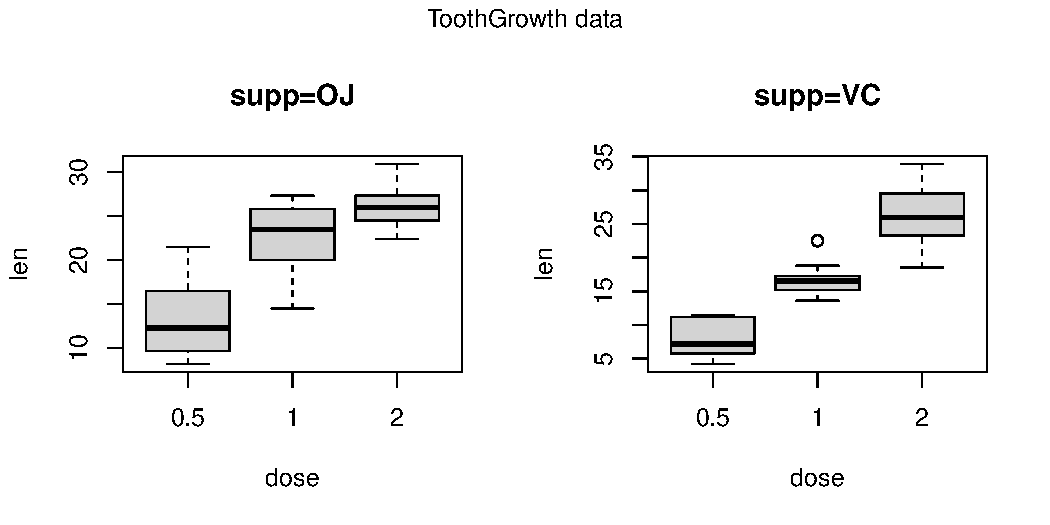
\includegraphics[width=\maxwidth]{figures/LSmeansunnamed-chunk-5-1} 

\end{knitrout}



\begin{knitrout}
\definecolor{shadecolor}{rgb}{0.969, 0.969, 0.969}\color{fgcolor}\begin{kframe}
\begin{alltt}
\hlkwd{with}\hlstd{(ToothGrowth,} \hlkwd{interaction.plot}\hlstd{(dose, supp, len))}
\end{alltt}
\end{kframe}
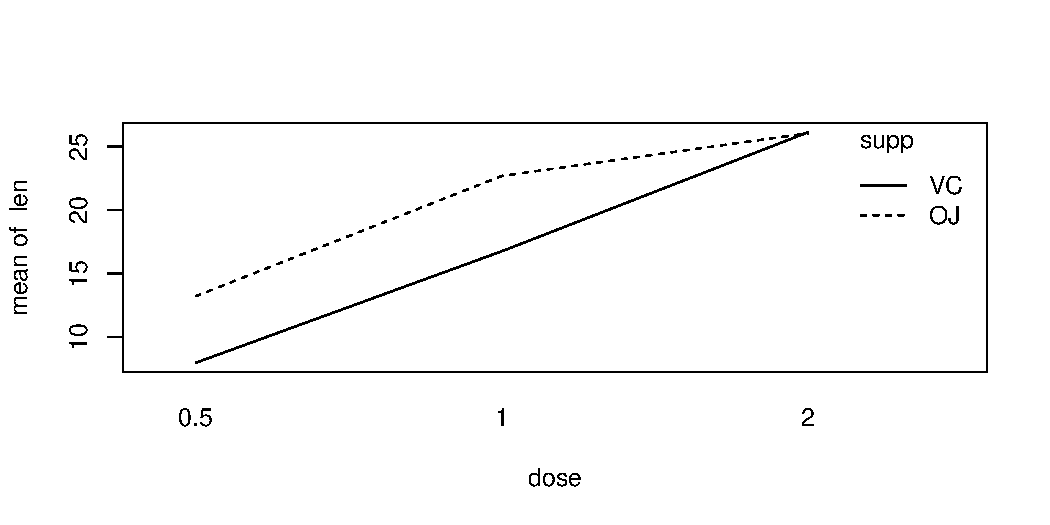
\includegraphics[width=\maxwidth]{figures/LSmeansunnamed-chunk-6-1} 

\end{knitrout}

The interaction plot suggests a mild interaction which is supported by a formal comparison:

\begin{knitrout}
\definecolor{shadecolor}{rgb}{0.969, 0.969, 0.969}\color{fgcolor}\begin{kframe}
\begin{alltt}
\hlstd{ToothGrowth}\hlopt{$}\hlstd{dose} \hlkwb{<-} \hlkwd{factor}\hlstd{(ToothGrowth}\hlopt{$}\hlstd{dose)}
\hlstd{tooth1} \hlkwb{<-} \hlkwd{lm}\hlstd{(len} \hlopt{~} \hlstd{dose} \hlopt{+} \hlstd{supp,} \hlkwc{data}\hlstd{=ToothGrowth)}
\hlstd{tooth2} \hlkwb{<-} \hlkwd{lm}\hlstd{(len} \hlopt{~} \hlstd{dose} \hlopt{*} \hlstd{supp,} \hlkwc{data}\hlstd{=ToothGrowth)}
\hlkwd{anova}\hlstd{(tooth1, tooth2)}
\end{alltt}
\begin{verbatim}
## Analysis of Variance Table
## 
## Model 1: len ~ dose + supp
## Model 2: len ~ dose * supp
##   Res.Df RSS Df Sum of Sq    F Pr(>F)  
## 1     56 820                           
## 2     54 712  2       108 4.11  0.022 *
## ---
## Signif. codes:  0 '***' 0.001 '**' 0.01 '*' 0.05 '.' 0.1 ' ' 1
\end{verbatim}
\end{kframe}
\end{knitrout}


\section{Computing linear estimates}
\label{sec:comp-line-estim}


For now, we focus on the additive model:
\begin{knitrout}
\definecolor{shadecolor}{rgb}{0.969, 0.969, 0.969}\color{fgcolor}\begin{kframe}
\begin{alltt}
\hlstd{tooth1}
\end{alltt}
\begin{verbatim}
## 
## Call:
## lm(formula = len ~ dose + supp, data = ToothGrowth)
## 
## Coefficients:
## (Intercept)        dose1        dose2       suppVC  
##       12.46         9.13        15.49        -3.70
\end{verbatim}
\end{kframe}
\end{knitrout}

The estimated length for each dose of orange juice (OJ) can be found
as follows. Notice: \verb|esticon| has been in the \doby\ package for
many years; \verb|linest| is a newer addition; \verb|esticon| is not
actively maintained but remains in \doby\ for historical reasons.



\begin{knitrout}
\definecolor{shadecolor}{rgb}{0.969, 0.969, 0.969}\color{fgcolor}\begin{kframe}
\begin{alltt}
\hlstd{L} \hlkwb{<-} \hlkwd{matrix}\hlstd{(}\hlkwd{c}\hlstd{(}\hlnum{1}\hlstd{,} \hlnum{0}\hlstd{,} \hlnum{0}\hlstd{,} \hlnum{0}\hlstd{,}
              \hlnum{1}\hlstd{,} \hlnum{1}\hlstd{,} \hlnum{0}\hlstd{,} \hlnum{0}\hlstd{,}
              \hlnum{1}\hlstd{,} \hlnum{0}\hlstd{,} \hlnum{1}\hlstd{,} \hlnum{0}\hlstd{),} \hlkwc{nrow}\hlstd{=}\hlnum{3}\hlstd{,} \hlkwc{byrow}\hlstd{=T)}
\hlstd{c1} \hlkwb{<-} \hlkwd{esticon}\hlstd{(tooth1, L)}
\hlstd{c1}
\end{alltt}
\begin{verbatim}
##       beta0 Estimate Std.Error t.value     DF Pr(>|t|)  Lower Upper
## [1,]  0.000   12.455     0.988  12.603 56.000    0.000 10.475  14.4
## [2,]  0.000   21.585     0.988  21.841 56.000    0.000 19.605  23.6
## [3,]  0.000   27.950     0.988  28.281 56.000    0.000 25.970  29.9
\end{verbatim}
\begin{alltt}
\hlstd{c2} \hlkwb{<-} \hlkwd{linest}\hlstd{(tooth1, L)}
\hlstd{c2}
\end{alltt}
\begin{verbatim}
## Coefficients:
##      estimate     se     df t.stat p.value
## [1,]   12.455  0.988 56.000 12.603       0
## [2,]   21.585  0.988 56.000 21.841       0
## [3,]   27.950  0.988 56.000 28.281       0
\end{verbatim}
\end{kframe}
\end{knitrout}



We can do:

\begin{knitrout}
\definecolor{shadecolor}{rgb}{0.969, 0.969, 0.969}\color{fgcolor}\begin{kframe}
\begin{alltt}
\hlkwd{summary}\hlstd{(c2)}
\end{alltt}
\begin{verbatim}
## Coefficients:
##      estimate     se     df t.stat p.value
## [1,]   12.455  0.988 56.000 12.603       0
## [2,]   21.585  0.988 56.000 21.841       0
## [3,]   27.950  0.988 56.000 28.281       0
## 
## Grid:
## NULL
## 
## L:
##      [,1] [,2] [,3] [,4]
## [1,]    1    0    0    0
## [2,]    1    1    0    0
## [3,]    1    0    1    0
\end{verbatim}
\begin{alltt}
\hlkwd{coef}\hlstd{(c2)}
\end{alltt}
\begin{verbatim}
##   estimate     se df t.stat   p.value
## 1    12.46 0.9883 56  12.60 5.490e-18
## 2    21.59 0.9883 56  21.84 4.461e-29
## 3    27.95 0.9883 56  28.28 7.627e-35
\end{verbatim}
\begin{alltt}
\hlkwd{confint}\hlstd{(c2)}
\end{alltt}
\begin{verbatim}
##   0.025 0.975
## 1 10.52 14.39
## 2 19.65 23.52
## 3 26.01 29.89
\end{verbatim}
\end{kframe}
\end{knitrout}

\section{Automatic generation of $L$}
\label{sec:autom-gener-l}



The matrix $L$ can be generated as follows:
\begin{knitrout}
\definecolor{shadecolor}{rgb}{0.969, 0.969, 0.969}\color{fgcolor}\begin{kframe}
\begin{alltt}
\hlstd{L} \hlkwb{<-} \hlkwd{linest_matrix}\hlstd{(tooth1,} \hlkwc{effect}\hlstd{=}\hlstr{"dose"}\hlstd{,} \hlkwc{at}\hlstd{=}\hlkwd{list}\hlstd{(}\hlkwc{supp}\hlstd{=}\hlstr{"OJ"}\hlstd{))}
\end{alltt}
\begin{verbatim}
## List of 8
##  $ effect        : chr "dose"
##  $ at            :List of 1
##   ..$ supp: chr "OJ"
##  $ fact.lev      :List of 2
##   ..$ dose: chr [1:3] "0.5" "1" "2"
##   ..$ supp: chr [1:2] "OJ" "VC"
##  $ new.fact.lev  :List of 2
##   ..$ dose: chr [1:3] "0.5" "1" "2"
##   ..$ supp: chr "OJ"
##  $ vartype       :List of 2
##   ..$ numeric: chr(0) 
##   ..$ factor : chr [1:2] "dose" "supp"
##  $ cov.ave       : Named list()
##   ..- attr(*, "at.num")= Named list()
##  $ at.factor.name: chr "supp"
##  $ cov.ave.name  : chr(0) 
## The general case; there are 'effect' factors or 'at' factors...
\end{verbatim}
\begin{alltt}
\hlstd{L}
\end{alltt}
\begin{verbatim}
##      (Intercept) dose1 dose2 suppVC
## [1,]           1     0     0      0
## [2,]           1     1     0      0
## [3,]           1     0     1      0
\end{verbatim}
\end{kframe}
\end{knitrout}

% << >>= 
% LSmeans(tooth1, effect="dose", at=list(supp="OJ"))
% @




\section{Least-squares means (LS--means)}
\label{sec:least-squares-means}

A special type of linear estimates is the so called least--squares
means (or LS--means). Other names for these estimates include
population means and marginal means. Notice that the \pkg{lsmeans} package
\cite{Lenth:2013} also provides computations of LS--means, see
\url{http://cran.r-project.org/web/packages/lsmeans/}.



\subsection{LS--means on a simple example}
\label{sec:ls-means-simple}

Consider these simulated data, also shown in Fig.~\ref{fig:simdat2-fig}:
\begin{knitrout}
\definecolor{shadecolor}{rgb}{0.969, 0.969, 0.969}\color{fgcolor}\begin{kframe}
\begin{alltt}
\hlstd{simdat}
\end{alltt}
\begin{verbatim}
##   treat year   y
## 1    t1    1 0.5
## 2    t1    1 1.0
## 3    t1    1 1.5
## 4    t2    1 3.0
## 5    t1    2 3.0
## 6    t2    2 4.5
## 7    t2    2 5.0
## 8    t2    2 5.5
\end{verbatim}
\end{kframe}
\end{knitrout}

\begin{knitrout}
\definecolor{shadecolor}{rgb}{0.969, 0.969, 0.969}\color{fgcolor}\begin{kframe}
\begin{alltt}
\hlkwd{library}\hlstd{(ggplot2)}
\hlkwd{qplot}\hlstd{(treat, y,} \hlkwc{data}\hlstd{=simdat,} \hlkwc{color}\hlstd{=year)}
\end{alltt}
\end{kframe}\begin{figure}
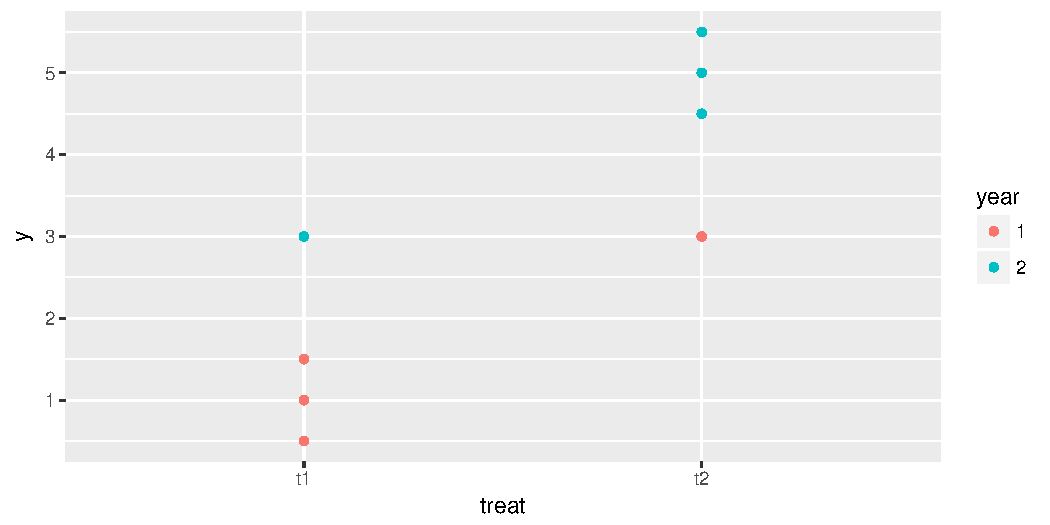
\includegraphics[width=\maxwidth]{figures/LSmeanssimdat2-fig-1} \caption[LSmeans - simulated data]{LSmeans - simulated data.}\label{fig:simdat2-fig}
\end{figure}


\end{knitrout}


The LS--means under an additive model for the factor \cc{treat} is the predicted outcome for each level of \cc{treat} for an ``average year'':
\begin{knitrout}
\definecolor{shadecolor}{rgb}{0.969, 0.969, 0.969}\color{fgcolor}\begin{kframe}
\begin{alltt}
\hlstd{msim} \hlkwb{<-} \hlkwd{lm}\hlstd{(y} \hlopt{~} \hlstd{treat} \hlopt{+} \hlstd{year,} \hlkwc{data}\hlstd{=simdat)}
\hlstd{lsm} \hlkwb{<-} \hlkwd{LSmeans}\hlstd{(msim,} \hlkwc{effect}\hlstd{=}\hlstr{"treat"}\hlstd{)}
\end{alltt}
\begin{verbatim}
## List of 8
##  $ effect        : chr "treat"
##  $ at            : NULL
##  $ fact.lev      :List of 2
##   ..$ treat: chr [1:2] "t1" "t2"
##   ..$ year : chr [1:2] "1" "2"
##  $ new.fact.lev  :List of 1
##   ..$ treat: chr [1:2] "t1" "t2"
##  $ vartype       :List of 2
##   ..$ numeric: chr(0) 
##   ..$ factor : chr [1:2] "treat" "year"
##  $ cov.ave       : Named list()
##  $ at.factor.name: NULL
##  $ cov.ave.name  : chr(0) 
## The general case; there are 'effect' factors or 'at' factors...
\end{verbatim}
\begin{alltt}
\hlstd{lsm}
\end{alltt}
\begin{verbatim}
## Coefficients:
##      estimate     se     df t.stat p.value
## [1,]    2.000  0.242  5.000  8.281       0
## [2,]    4.000  0.242  5.000 16.562       0
\end{verbatim}
\end{kframe}
\end{knitrout}


Notice that the population means are
\begin{knitrout}
\definecolor{shadecolor}{rgb}{0.969, 0.969, 0.969}\color{fgcolor}\begin{kframe}
\begin{alltt}
\hlkwd{summaryBy}\hlstd{(y} \hlopt{~} \hlstd{treat,} \hlkwc{data}\hlstd{=simdat,} \hlkwc{FUN}\hlstd{=}\hlkwa{function}\hlstd{(}\hlkwc{x}\hlstd{)} \hlkwd{c}\hlstd{(}\hlkwc{m}\hlstd{=}\hlkwd{mean}\hlstd{(x),} \hlkwc{s}\hlstd{=}\hlkwd{sd}\hlstd{(x)))}
\end{alltt}
\begin{verbatim}
##   treat  y.m  y.s
## 1    t1 1.50 1.08
## 2    t2 4.50 1.08
\end{verbatim}
\begin{alltt}
\hlcom{## or aggregate(y ~ treat, data=simdat, FUN=function(x) c(m=mean(x), s=sd(x)))}
\end{alltt}
\end{kframe}
\end{knitrout}

Had data been balanced (same number of observations for each
combination of \cc{treat} and \cc{year}) the results would have been the
same. An argument in favor of the LS--means is that these figures
better represent what one would expect on in an ``average year''.

An alternative is to think of  \cc{year} as a random
effect, for example:
\begin{knitrout}
\definecolor{shadecolor}{rgb}{0.969, 0.969, 0.969}\color{fgcolor}\begin{kframe}
\begin{alltt}
\hlkwd{library}\hlstd{(lme4)}
\hlkwd{lmer}\hlstd{( y} \hlopt{~} \hlstd{treat}  \hlopt{+} \hlstd{(}\hlnum{1}\hlopt{|}\hlstd{year),} \hlkwc{data}\hlstd{=simdat)}
\end{alltt}
\end{kframe}
\end{knitrout}

In this case one would directly obtain $\EE(Y|\cc{treat})$ from the
model. However, there are at least two reasons why one may be hesitant
to consider such a random effects model.
\begin{itemize}
\item It is a ``never ending'' discussion whether \verb|year| should
  be treated as fixed or random. For \verb|year| to be a random
  effect, it should in principle come from a large population of
  possible years. This is certainly a dubious assumption for the
  years.
\item If we accept to think of year as a random effect, then the
  variance describing this random effect will be poorly determined
  (because there are only two years in the study).
\end{itemize}

\subsection{Additive model}
\label{sec:additive-model}


Returning to the \verb|ToothGrowth| data, orange juice and ascorbic
acid are just two of many ways of supplying vitamin C (citrus and lime
juice would be two alternatives). Here one can therefore argue, that
it would make sense to estimate the the effect for each dose for an
``average vitamin C source'':

\begin{knitrout}
\definecolor{shadecolor}{rgb}{0.969, 0.969, 0.969}\color{fgcolor}\begin{kframe}
\begin{alltt}
\hlkwd{LSmeans}\hlstd{(tooth1,} \hlkwc{effect}\hlstd{=}\hlstr{"dose"}\hlstd{)}
\end{alltt}
\begin{verbatim}
## List of 8
##  $ effect        : chr "dose"
##  $ at            : NULL
##  $ fact.lev      :List of 2
##   ..$ dose: chr [1:3] "0.5" "1" "2"
##   ..$ supp: chr [1:2] "OJ" "VC"
##  $ new.fact.lev  :List of 1
##   ..$ dose: chr [1:3] "0.5" "1" "2"
##  $ vartype       :List of 2
##   ..$ numeric: chr(0) 
##   ..$ factor : chr [1:2] "dose" "supp"
##  $ cov.ave       : Named list()
##  $ at.factor.name: NULL
##  $ cov.ave.name  : chr(0) 
## The general case; there are 'effect' factors or 'at' factors...
## Coefficients:
##      estimate     se     df t.stat p.value
## [1,]   10.605  0.856 56.000 12.391       0
## [2,]   19.735  0.856 56.000 23.058       0
## [3,]   26.100  0.856 56.000 30.495       0
\end{verbatim}
\end{kframe}
\end{knitrout}

which is the same as
\begin{knitrout}
\definecolor{shadecolor}{rgb}{0.969, 0.969, 0.969}\color{fgcolor}\begin{kframe}
\begin{alltt}
\hlstd{L} \hlkwb{<-} \hlkwd{linest_matrix}\hlstd{(tooth1,} \hlkwc{effect}\hlstd{=}\hlstr{"dose"}\hlstd{)}
\end{alltt}
\begin{verbatim}
## List of 8
##  $ effect        : chr "dose"
##  $ at            : NULL
##  $ fact.lev      :List of 2
##   ..$ dose: chr [1:3] "0.5" "1" "2"
##   ..$ supp: chr [1:2] "OJ" "VC"
##  $ new.fact.lev  :List of 1
##   ..$ dose: chr [1:3] "0.5" "1" "2"
##  $ vartype       :List of 2
##   ..$ numeric: chr(0) 
##   ..$ factor : chr [1:2] "dose" "supp"
##  $ cov.ave       : Named list()
##  $ at.factor.name: NULL
##  $ cov.ave.name  : chr(0) 
## The general case; there are 'effect' factors or 'at' factors...
\end{verbatim}
\begin{alltt}
\hlstd{L}
\end{alltt}
\begin{verbatim}
##      (Intercept) dose1 dose2 suppVC
## [1,]           1     0     0    0.5
## [2,]           1     1     0    0.5
## [3,]           1     0     1    0.5
\end{verbatim}
\begin{alltt}
\hlstd{le} \hlkwb{<-} \hlkwd{linest}\hlstd{(tooth1,} \hlkwc{L}\hlstd{=L)}
\hlkwd{coef}\hlstd{(le)}
\end{alltt}
\begin{verbatim}
##   estimate     se df t.stat   p.value
## 1    10.61 0.8559 56  12.39 1.109e-17
## 2    19.73 0.8559 56  23.06 2.885e-30
## 3    26.10 0.8559 56  30.50 1.444e-36
\end{verbatim}
\end{kframe}
\end{knitrout}

\subsection{Interaction model}
\label{sec:interaction-model}


For a model with interactions, the LSmeans are
\begin{knitrout}
\definecolor{shadecolor}{rgb}{0.969, 0.969, 0.969}\color{fgcolor}\begin{kframe}
\begin{alltt}
\hlkwd{LSmeans}\hlstd{(tooth2,} \hlkwc{effect}\hlstd{=}\hlstr{"dose"}\hlstd{)}
\end{alltt}
\begin{verbatim}
## List of 8
##  $ effect        : chr "dose"
##  $ at            : NULL
##  $ fact.lev      :List of 2
##   ..$ dose: chr [1:3] "0.5" "1" "2"
##   ..$ supp: chr [1:2] "OJ" "VC"
##  $ new.fact.lev  :List of 1
##   ..$ dose: chr [1:3] "0.5" "1" "2"
##  $ vartype       :List of 2
##   ..$ numeric: chr(0) 
##   ..$ factor : chr [1:2] "dose" "supp"
##  $ cov.ave       : Named list()
##  $ at.factor.name: NULL
##  $ cov.ave.name  : chr(0) 
## The general case; there are 'effect' factors or 'at' factors...
## Coefficients:
##      estimate     se     df t.stat p.value
## [1,]   10.605  0.812 54.000 13.060       0
## [2,]   19.735  0.812 54.000 24.304       0
## [3,]   26.100  0.812 54.000 32.143       0
\end{verbatim}
\end{kframe}
\end{knitrout}

In this case, the $L$ matrix is
\begin{knitrout}
\definecolor{shadecolor}{rgb}{0.969, 0.969, 0.969}\color{fgcolor}\begin{kframe}
\begin{alltt}
\hlstd{L} \hlkwb{<-} \hlkwd{linest_matrix}\hlstd{(tooth2,} \hlkwc{effect}\hlstd{=}\hlstr{"dose"}\hlstd{)}
\end{alltt}
\begin{verbatim}
## List of 8
##  $ effect        : chr "dose"
##  $ at            : NULL
##  $ fact.lev      :List of 2
##   ..$ dose: chr [1:3] "0.5" "1" "2"
##   ..$ supp: chr [1:2] "OJ" "VC"
##  $ new.fact.lev  :List of 1
##   ..$ dose: chr [1:3] "0.5" "1" "2"
##  $ vartype       :List of 2
##   ..$ numeric: chr(0) 
##   ..$ factor : chr [1:2] "dose" "supp"
##  $ cov.ave       : Named list()
##  $ at.factor.name: NULL
##  $ cov.ave.name  : chr(0) 
## The general case; there are 'effect' factors or 'at' factors...
\end{verbatim}
\begin{alltt}
\hlkwd{t}\hlstd{(L)}
\end{alltt}
\begin{verbatim}
##              [,1] [,2] [,3]
## (Intercept)   1.0  1.0  1.0
## dose1         0.0  1.0  0.0
## dose2         0.0  0.0  1.0
## suppVC        0.5  0.5  0.5
## dose1:suppVC  0.0  0.5  0.0
## dose2:suppVC  0.0  0.0  0.5
\end{verbatim}
\end{kframe}
\end{knitrout}



















\section{Using the \code{at=} argument}
\label{sec:example:-chickweight}


\begin{knitrout}
\definecolor{shadecolor}{rgb}{0.969, 0.969, 0.969}\color{fgcolor}\begin{kframe}
\begin{alltt}
\hlkwd{library}\hlstd{(ggplot2)}
\hlstd{ChickWeight}\hlopt{$}\hlstd{Diet} \hlkwb{<-} \hlkwd{factor}\hlstd{(ChickWeight}\hlopt{$}\hlstd{Diet)}
\hlkwd{qplot}\hlstd{(Time, weight,} \hlkwc{data}\hlstd{=ChickWeight,} \hlkwc{colour}\hlstd{=Chick,} \hlkwc{facets}\hlstd{=}\hlopt{~}\hlstd{Diet,}
      \hlkwc{geom}\hlstd{=}\hlkwd{c}\hlstd{(}\hlstr{"point"}\hlstd{,}\hlstr{"line"}\hlstd{))}
\end{alltt}
\end{kframe}\begin{figure}
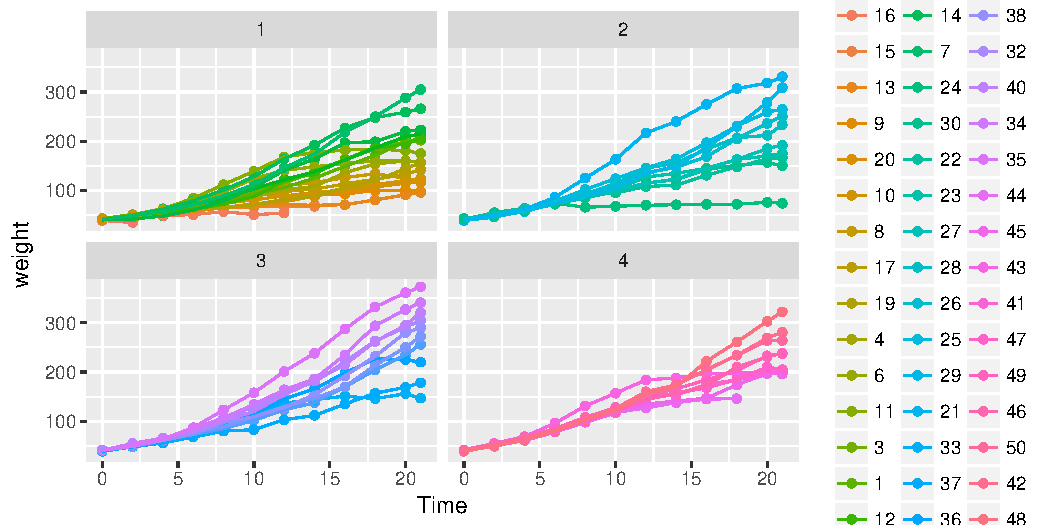
\includegraphics[width=\maxwidth]{figures/LSmeanschick-fig-1} \caption[ChickWeight data]{ChickWeight data.}\label{fig:chick-fig}
\end{figure}


\end{knitrout}

Consider random regression model:
\begin{knitrout}
\definecolor{shadecolor}{rgb}{0.969, 0.969, 0.969}\color{fgcolor}\begin{kframe}
\begin{alltt}
\hlkwd{library}\hlstd{(lme4)}
\hlstd{chick} \hlkwb{<-} \hlkwd{lmer}\hlstd{(weight} \hlopt{~} \hlstd{Time} \hlopt{*} \hlstd{Diet} \hlopt{+} \hlstd{(}\hlnum{0} \hlopt{+} \hlstd{Time} \hlopt{|} \hlstd{Chick),}
           \hlkwc{data}\hlstd{=ChickWeight)}
\hlkwd{coef}\hlstd{(}\hlkwd{summary}\hlstd{(chick))}
\end{alltt}
\begin{verbatim}
##             Estimate Std. Error t value
## (Intercept)   33.218     1.7697 18.7701
## Time           6.339     0.6103 10.3855
## Diet2         -4.585     3.0047 -1.5258
## Diet3        -14.968     3.0047 -4.9815
## Diet4         -1.454     3.0177 -0.4818
## Time:Diet2     2.271     1.0367  2.1902
## Time:Diet3     5.084     1.0367  4.9043
## Time:Diet4     3.217     1.0377  3.1004
\end{verbatim}
\end{kframe}
\end{knitrout}


The contrast matrix for \cc{Diet} becomes:
\begin{knitrout}
\definecolor{shadecolor}{rgb}{0.969, 0.969, 0.969}\color{fgcolor}\begin{kframe}
\begin{alltt}
\hlstd{L} \hlkwb{<-} \hlkwd{linest_matrix}\hlstd{(chick,} \hlkwc{effect}\hlstd{=}\hlstr{"Diet"}\hlstd{)}
\end{alltt}
\begin{verbatim}
## List of 8
##  $ effect        : chr "Diet"
##  $ at            : NULL
##  $ fact.lev      :List of 1
##   ..$ Diet: chr [1:4] "1" "2" "3" "4"
##  $ new.fact.lev  :List of 1
##   ..$ Diet: chr [1:4] "1" "2" "3" "4"
##  $ vartype       :List of 2
##   ..$ numeric: chr "Time"
##   ..$ factor : chr "Diet"
##  $ cov.ave       :List of 1
##   ..$ Time: num 10.7
##  $ at.factor.name: NULL
##  $ cov.ave.name  : chr "Time"
## The general case; there are 'effect' factors or 'at' factors...
\end{verbatim}
\begin{alltt}
\hlkwd{t}\hlstd{(L)}
\end{alltt}
\begin{verbatim}
##              [,1]  [,2]  [,3]  [,4]
## (Intercept)  1.00  1.00  1.00  1.00
## Time        10.72 10.72 10.72 10.72
## Diet2        0.00  1.00  0.00  0.00
## Diet3        0.00  0.00  1.00  0.00
## Diet4        0.00  0.00  0.00  1.00
## Time:Diet2   0.00 10.72  0.00  0.00
## Time:Diet3   0.00  0.00 10.72  0.00
## Time:Diet4   0.00  0.00  0.00 10.72
\end{verbatim}
\end{kframe}
\end{knitrout}

The value of \cc{Time} is by default taken to be the average of that
variable. Hence the \lsmeans\ is the predicted weight for each diet at
that specific point of time. We can consider other points of time with
\begin{knitrout}
\definecolor{shadecolor}{rgb}{0.969, 0.969, 0.969}\color{fgcolor}\begin{kframe}
\begin{alltt}
\hlstd{K1} \hlkwb{<-} \hlkwd{linest_matrix}\hlstd{(chick,} \hlkwc{effect}\hlstd{=}\hlstr{"Diet"}\hlstd{,} \hlkwc{at}\hlstd{=}\hlkwd{list}\hlstd{(}\hlkwc{Time}\hlstd{=}\hlnum{1}\hlstd{))}
\end{alltt}
\begin{verbatim}
## List of 8
##  $ effect        : chr "Diet"
##  $ at            :List of 1
##   ..$ Time: num 1
##  $ fact.lev      :List of 1
##   ..$ Diet: chr [1:4] "1" "2" "3" "4"
##  $ new.fact.lev  :List of 1
##   ..$ Diet: chr [1:4] "1" "2" "3" "4"
##  $ vartype       :List of 2
##   ..$ numeric: chr "Time"
##   ..$ factor : chr "Diet"
##  $ cov.ave       :List of 1
##   ..$ Time: num 1
##   ..- attr(*, "at.num")=List of 1
##   .. ..$ Time: num 1
##  $ at.factor.name: chr(0) 
##  $ cov.ave.name  : chr "Time"
## The general case; there are 'effect' factors or 'at' factors...
\end{verbatim}
\begin{alltt}
\hlkwd{t}\hlstd{(K1)}
\end{alltt}
\begin{verbatim}
##             [,1] [,2] [,3] [,4]
## (Intercept)    1    1    1    1
## Time           1    1    1    1
## Diet2          0    1    0    0
## Diet3          0    0    1    0
## Diet4          0    0    0    1
## Time:Diet2     0    1    0    0
## Time:Diet3     0    0    1    0
## Time:Diet4     0    0    0    1
\end{verbatim}
\end{kframe}
\end{knitrout}

The \lsmeans\ for the intercepts is the predictions at
\cc{Time=0}. The \lsmeans\ for the slopes becomes
\begin{knitrout}
\definecolor{shadecolor}{rgb}{0.969, 0.969, 0.969}\color{fgcolor}\begin{kframe}
\begin{alltt}
\hlstd{K0} \hlkwb{<-} \hlkwd{linest_matrix}\hlstd{(chick,} \hlkwc{effect}\hlstd{=}\hlstr{"Diet"}\hlstd{,} \hlkwc{at}\hlstd{=}\hlkwd{list}\hlstd{(}\hlkwc{Time}\hlstd{=}\hlnum{0}\hlstd{))}
\end{alltt}
\begin{verbatim}
## List of 8
##  $ effect        : chr "Diet"
##  $ at            :List of 1
##   ..$ Time: num 0
##  $ fact.lev      :List of 1
##   ..$ Diet: chr [1:4] "1" "2" "3" "4"
##  $ new.fact.lev  :List of 1
##   ..$ Diet: chr [1:4] "1" "2" "3" "4"
##  $ vartype       :List of 2
##   ..$ numeric: chr "Time"
##   ..$ factor : chr "Diet"
##  $ cov.ave       :List of 1
##   ..$ Time: num 0
##   ..- attr(*, "at.num")=List of 1
##   .. ..$ Time: num 0
##  $ at.factor.name: chr(0) 
##  $ cov.ave.name  : chr "Time"
## The general case; there are 'effect' factors or 'at' factors...
\end{verbatim}
\begin{alltt}
\hlkwd{t}\hlstd{(K1} \hlopt{-} \hlstd{K0)}
\end{alltt}
\begin{verbatim}
##             [,1] [,2] [,3] [,4]
## (Intercept)    0    0    0    0
## Time           1    1    1    1
## Diet2          0    0    0    0
## Diet3          0    0    0    0
## Diet4          0    0    0    0
## Time:Diet2     0    1    0    0
## Time:Diet3     0    0    1    0
## Time:Diet4     0    0    0    1
\end{verbatim}
\begin{alltt}
\hlkwd{linest}\hlstd{(chick,} \hlkwc{L}\hlstd{=K1}\hlopt{-}\hlstd{K0)}
\end{alltt}
\begin{verbatim}
## Coefficients:
##      estimate     se     df t.stat p.value
## [1,]    6.339  0.610 49.855 10.383       0
## [2,]    8.609  0.838 48.282 10.273       0
## [3,]   11.423  0.838 48.282 13.631       0
## [4,]    9.556  0.839 48.565 11.386       0
\end{verbatim}
\end{kframe}
\end{knitrout}

We can cook up our own function for comparing trends:
\begin{knitrout}
\definecolor{shadecolor}{rgb}{0.969, 0.969, 0.969}\color{fgcolor}\begin{kframe}
\begin{alltt}
\hlstd{LSmeans_trend} \hlkwb{<-} \hlkwa{function}\hlstd{(}\hlkwc{object}\hlstd{,} \hlkwc{effect}\hlstd{,} \hlkwc{trend}\hlstd{)\{}

    \hlstd{K}\hlkwb{<-}\hlkwd{linest_matrix}\hlstd{(object,} \hlkwc{effect}\hlstd{=effect,} \hlkwc{at}\hlstd{=}\hlkwd{as.list}\hlstd{(}\hlkwd{setNames}\hlstd{(}\hlnum{1}\hlstd{, trend)))} \hlopt{-}
        \hlkwd{linest_matrix}\hlstd{(object,} \hlkwc{effect}\hlstd{=effect,} \hlkwc{at}\hlstd{=}\hlkwd{as.list}\hlstd{(}\hlkwd{setNames}\hlstd{(}\hlnum{0}\hlstd{, trend)))}
    \hlkwd{linest}\hlstd{(object,} \hlkwc{L}\hlstd{=K)}
\hlstd{\}}
\hlkwd{LSmeans_trend}\hlstd{(chick,} \hlkwc{effect}\hlstd{=}\hlstr{"Diet"}\hlstd{,} \hlkwc{trend}\hlstd{=}\hlstr{"Time"}\hlstd{)}
\end{alltt}
\begin{verbatim}
## List of 8
##  $ effect        : chr "Diet"
##  $ at            :List of 1
##   ..$ Time: num 1
##  $ fact.lev      :List of 1
##   ..$ Diet: chr [1:4] "1" "2" "3" "4"
##  $ new.fact.lev  :List of 1
##   ..$ Diet: chr [1:4] "1" "2" "3" "4"
##  $ vartype       :List of 2
##   ..$ numeric: chr "Time"
##   ..$ factor : chr "Diet"
##  $ cov.ave       :List of 1
##   ..$ Time: num 1
##   ..- attr(*, "at.num")=List of 1
##   .. ..$ Time: num 1
##  $ at.factor.name: chr(0) 
##  $ cov.ave.name  : chr "Time"
## The general case; there are 'effect' factors or 'at' factors...
## List of 8
##  $ effect        : chr "Diet"
##  $ at            :List of 1
##   ..$ Time: num 0
##  $ fact.lev      :List of 1
##   ..$ Diet: chr [1:4] "1" "2" "3" "4"
##  $ new.fact.lev  :List of 1
##   ..$ Diet: chr [1:4] "1" "2" "3" "4"
##  $ vartype       :List of 2
##   ..$ numeric: chr "Time"
##   ..$ factor : chr "Diet"
##  $ cov.ave       :List of 1
##   ..$ Time: num 0
##   ..- attr(*, "at.num")=List of 1
##   .. ..$ Time: num 0
##  $ at.factor.name: chr(0) 
##  $ cov.ave.name  : chr "Time"
## The general case; there are 'effect' factors or 'at' factors...
## Coefficients:
##      estimate     se     df t.stat p.value
## [1,]    6.339  0.610 49.855 10.383       0
## [2,]    8.609  0.838 48.282 10.273       0
## [3,]   11.423  0.838 48.282 13.631       0
## [4,]    9.556  0.839 48.565 11.386       0
\end{verbatim}
\end{kframe}
\end{knitrout}

\section{Using (transformed) covariates}
\label{sec:using-covariates}

Consider the following subset of the \code{CO2} dataset:
\begin{knitrout}
\definecolor{shadecolor}{rgb}{0.969, 0.969, 0.969}\color{fgcolor}\begin{kframe}
\begin{alltt}
\hlkwd{data}\hlstd{(CO2)}
\hlstd{CO2} \hlkwb{<-} \hlkwd{transform}\hlstd{(CO2,} \hlkwc{Treat}\hlstd{=Treatment,} \hlkwc{Treatment}\hlstd{=}\hlkwa{NULL}\hlstd{)}
\hlkwd{levels}\hlstd{(CO2}\hlopt{$}\hlstd{Treat)} \hlkwb{<-} \hlkwd{c}\hlstd{(}\hlstr{"nchil"}\hlstd{,}\hlstr{"chil"}\hlstd{)}
\hlkwd{levels}\hlstd{(CO2}\hlopt{$}\hlstd{Type)} \hlkwb{<-} \hlkwd{c}\hlstd{(}\hlstr{"Que"}\hlstd{,}\hlstr{"Mis"}\hlstd{)}
\hlkwd{ftable}\hlstd{(}\hlkwd{xtabs}\hlstd{(} \hlopt{~} \hlstd{Plant} \hlopt{+} \hlstd{Type} \hlopt{+} \hlstd{Treat,} \hlkwc{data}\hlstd{=CO2),} \hlkwc{col.vars}\hlstd{=}\hlnum{2}\hlopt{:}\hlnum{3}\hlstd{)}
\end{alltt}
\begin{verbatim}
##       Type    Que        Mis     
##       Treat nchil chil nchil chil
## Plant                            
## Qn1             7    0     0    0
## Qn2             7    0     0    0
## Qn3             7    0     0    0
## Qc1             0    7     0    0
## Qc3             0    7     0    0
## Qc2             0    7     0    0
## Mn3             0    0     7    0
## Mn2             0    0     7    0
## Mn1             0    0     7    0
## Mc2             0    0     0    7
## Mc3             0    0     0    7
## Mc1             0    0     0    7
\end{verbatim}
\end{kframe}
\end{knitrout}

\begin{knitrout}
\definecolor{shadecolor}{rgb}{0.969, 0.969, 0.969}\color{fgcolor}\begin{kframe}
\begin{alltt}
\hlkwd{qplot}\hlstd{(}\hlkwc{x}\hlstd{=}\hlkwd{log}\hlstd{(conc),} \hlkwc{y}\hlstd{=uptake,} \hlkwc{data}\hlstd{=CO2,} \hlkwc{color}\hlstd{=Treat,} \hlkwc{facets}\hlstd{=}\hlopt{~}\hlstd{Type)}
\end{alltt}
\end{kframe}\begin{figure}
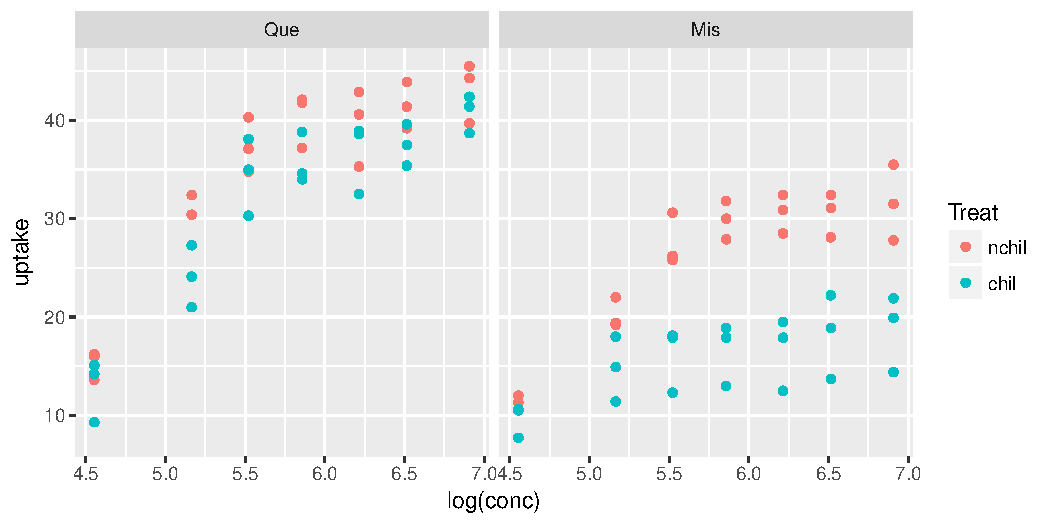
\includegraphics[width=\maxwidth]{figures/LSmeansco2-fig-1} \caption[CO2 data]{CO2 data}\label{fig:co2-fig}
\end{figure}


\end{knitrout}
%%\includegraphics[height=6cm,width=12cm]{figures/LSmeans-co2-fig}

Below, the covariate \code{conc} is fixed at the average value:
\begin{knitrout}
\definecolor{shadecolor}{rgb}{0.969, 0.969, 0.969}\color{fgcolor}\begin{kframe}
\begin{alltt}
\hlstd{co2.lm1} \hlkwb{<-} \hlkwd{lm}\hlstd{(uptake} \hlopt{~} \hlstd{conc} \hlopt{+} \hlstd{Type} \hlopt{+} \hlstd{Treat,} \hlkwc{data}\hlstd{=CO2)}
\hlkwd{LSmeans}\hlstd{(co2.lm1,} \hlkwc{effect}\hlstd{=}\hlstr{"Treat"}\hlstd{)}
\end{alltt}
\begin{verbatim}
## List of 8
##  $ effect        : chr "Treat"
##  $ at            : NULL
##  $ fact.lev      :List of 2
##   ..$ Type : chr [1:2] "Que" "Mis"
##   ..$ Treat: chr [1:2] "nchil" "chil"
##  $ new.fact.lev  :List of 1
##   ..$ Treat: chr [1:2] "nchil" "chil"
##  $ vartype       :List of 2
##   ..$ numeric: chr "conc"
##   ..$ factor : chr [1:2] "Type" "Treat"
##  $ cov.ave       :List of 1
##   ..$ conc: num 435
##  $ at.factor.name: NULL
##  $ cov.ave.name  : chr "conc"
## The general case; there are 'effect' factors or 'at' factors...
## Coefficients:
##      estimate     se     df t.stat p.value
## [1,]   30.643  0.956 80.000 32.066       0
## [2,]   23.783  0.956 80.000 24.888       0
\end{verbatim}
\end{kframe}
\end{knitrout}

If we use \code{log(conc)} instead we will get an error when
calculating LS--means:
\begin{knitrout}
\definecolor{shadecolor}{rgb}{0.969, 0.969, 0.969}\color{fgcolor}\begin{kframe}
\begin{alltt}
\hlstd{co2.lm} \hlkwb{<-} \hlkwd{lm}\hlstd{(uptake} \hlopt{~} \hlkwd{log}\hlstd{(conc)} \hlopt{+} \hlstd{Type} \hlopt{+} \hlstd{Treat,} \hlkwc{data}\hlstd{=CO2)}
\hlkwd{LSmeans}\hlstd{(co2.lm,} \hlkwc{effect}\hlstd{=}\hlstr{"Treat"}\hlstd{)}
\end{alltt}
\end{kframe}
\end{knitrout}

In this case one can do
\begin{knitrout}
\definecolor{shadecolor}{rgb}{0.969, 0.969, 0.969}\color{fgcolor}\begin{kframe}
\begin{alltt}
\hlstd{co2.lm2} \hlkwb{<-} \hlkwd{lm}\hlstd{(uptake} \hlopt{~} \hlstd{log.conc} \hlopt{+} \hlstd{Type} \hlopt{+} \hlstd{Treat,}
             \hlkwc{data}\hlstd{=}\hlkwd{transform}\hlstd{(CO2,} \hlkwc{log.conc}\hlstd{=}\hlkwd{log}\hlstd{(conc)))}
\hlkwd{LSmeans}\hlstd{(co2.lm2,} \hlkwc{effect}\hlstd{=}\hlstr{"Treat"}\hlstd{)}
\end{alltt}
\begin{verbatim}
## List of 8
##  $ effect        : chr "Treat"
##  $ at            : NULL
##  $ fact.lev      :List of 2
##   ..$ Type : chr [1:2] "Que" "Mis"
##   ..$ Treat: chr [1:2] "nchil" "chil"
##  $ new.fact.lev  :List of 1
##   ..$ Treat: chr [1:2] "nchil" "chil"
##  $ vartype       :List of 2
##   ..$ numeric: chr "log.conc"
##   ..$ factor : chr [1:2] "Type" "Treat"
##  $ cov.ave       :List of 1
##   ..$ log.conc: num 5.82
##  $ at.factor.name: NULL
##  $ cov.ave.name  : chr "log.conc"
## The general case; there are 'effect' factors or 'at' factors...
## Coefficients:
##      estimate     se     df t.stat p.value
## [1,]   30.643  0.761 80.000 40.261       0
## [2,]   23.783  0.761 80.000 31.248       0
\end{verbatim}
\end{kframe}
\end{knitrout}
This also highlights what is computed: The average of the log of
\code{conc}; not the log of the average of \code{conc}.

In a similar spirit consider
\begin{knitrout}
\definecolor{shadecolor}{rgb}{0.969, 0.969, 0.969}\color{fgcolor}\begin{kframe}
\begin{alltt}
\hlstd{co2.lm3} \hlkwb{<-} \hlkwd{lm}\hlstd{(uptake} \hlopt{~} \hlstd{conc} \hlopt{+} \hlkwd{I}\hlstd{(conc}\hlopt{^}\hlnum{2}\hlstd{)} \hlopt{+} \hlstd{Type} \hlopt{+} \hlstd{Treat,} \hlkwc{data}\hlstd{=CO2)}
\hlkwd{LSmeans}\hlstd{(co2.lm3,} \hlkwc{effect}\hlstd{=}\hlstr{"Treat"}\hlstd{)}
\end{alltt}
\begin{verbatim}
## List of 8
##  $ effect        : chr "Treat"
##  $ at            : NULL
##  $ fact.lev      :List of 2
##   ..$ Type : chr [1:2] "Que" "Mis"
##   ..$ Treat: chr [1:2] "nchil" "chil"
##  $ new.fact.lev  :List of 1
##   ..$ Treat: chr [1:2] "nchil" "chil"
##  $ vartype       :List of 2
##   ..$ numeric: chr [1:2] "conc" "I(conc^2)"
##   ..$ factor : chr [1:2] "Type" "Treat"
##  $ cov.ave       :List of 2
##   ..$ conc     : num 435
##   ..$ I(conc^2): num 275754
##  $ at.factor.name: NULL
##  $ cov.ave.name  : chr [1:2] "conc" "I(conc^2)"
## The general case; there are 'effect' factors or 'at' factors...
## Coefficients:
##      estimate     se     df t.stat p.value
## [1,]   34.543  0.982 79.000 35.191       0
## [2,]   27.683  0.982 79.000 28.202       0
\end{verbatim}
\end{kframe}
\end{knitrout}

Above \verb'I(conc^2)' is the average of the squared values of
\code{conc}; not the  square of the average of
\code{conc}, cfr.\ the following.

\begin{knitrout}
\definecolor{shadecolor}{rgb}{0.969, 0.969, 0.969}\color{fgcolor}\begin{kframe}
\begin{alltt}
\hlstd{co2.lm4} \hlkwb{<-} \hlkwd{lm}\hlstd{(uptake} \hlopt{~} \hlstd{conc} \hlopt{+} \hlstd{conc2} \hlopt{+} \hlstd{Type} \hlopt{+} \hlstd{Treat,} \hlkwc{data}\hlstd{=}
              \hlkwd{transform}\hlstd{(CO2,} \hlkwc{conc2}\hlstd{=conc}\hlopt{^}\hlnum{2}\hlstd{))}
\hlkwd{LSmeans}\hlstd{(co2.lm4,} \hlkwc{effect}\hlstd{=}\hlstr{"Treat"}\hlstd{)}
\end{alltt}
\begin{verbatim}
## List of 8
##  $ effect        : chr "Treat"
##  $ at            : NULL
##  $ fact.lev      :List of 2
##   ..$ Type : chr [1:2] "Que" "Mis"
##   ..$ Treat: chr [1:2] "nchil" "chil"
##  $ new.fact.lev  :List of 1
##   ..$ Treat: chr [1:2] "nchil" "chil"
##  $ vartype       :List of 2
##   ..$ numeric: chr [1:2] "conc" "conc2"
##   ..$ factor : chr [1:2] "Type" "Treat"
##  $ cov.ave       :List of 2
##   ..$ conc : num 435
##   ..$ conc2: num 275754
##  $ at.factor.name: NULL
##  $ cov.ave.name  : chr [1:2] "conc" "conc2"
## The general case; there are 'effect' factors or 'at' factors...
## Coefficients:
##      estimate     se     df t.stat p.value
## [1,]   30.643  0.776 79.000 39.465       0
## [2,]   23.783  0.776 79.000 30.630       0
\end{verbatim}
\end{kframe}
\end{knitrout}

If we want to evaluate the LS--means at \code{conc=10} then we can do:
\begin{knitrout}
\definecolor{shadecolor}{rgb}{0.969, 0.969, 0.969}\color{fgcolor}\begin{kframe}
\begin{alltt}
\hlkwd{LSmeans}\hlstd{(co2.lm4,} \hlkwc{effect}\hlstd{=}\hlstr{"Treat"}\hlstd{,} \hlkwc{at}\hlstd{=}\hlkwd{list}\hlstd{(}\hlkwc{conc}\hlstd{=}\hlnum{10}\hlstd{,} \hlkwc{conc2}\hlstd{=}\hlnum{100}\hlstd{))}
\end{alltt}
\begin{verbatim}
## List of 8
##  $ effect        : chr "Treat"
##  $ at            :List of 2
##   ..$ conc : num 10
##   ..$ conc2: num 100
##  $ fact.lev      :List of 2
##   ..$ Type : chr [1:2] "Que" "Mis"
##   ..$ Treat: chr [1:2] "nchil" "chil"
##  $ new.fact.lev  :List of 1
##   ..$ Treat: chr [1:2] "nchil" "chil"
##  $ vartype       :List of 2
##   ..$ numeric: chr [1:2] "conc" "conc2"
##   ..$ factor : chr [1:2] "Type" "Treat"
##  $ cov.ave       :List of 2
##   ..$ conc : num 10
##   ..$ conc2: num 100
##   ..- attr(*, "at.num")=List of 2
##   .. ..$ conc : num 10
##   .. ..$ conc2: num 100
##  $ at.factor.name: chr(0) 
##  $ cov.ave.name  : chr [1:2] "conc" "conc2"
## The general case; there are 'effect' factors or 'at' factors...
## Coefficients:
##      estimate    se    df t.stat p.value
## [1,]    14.74  1.70 79.00   8.66       0
## [2,]     7.88  1.70 79.00   4.63       0
\end{verbatim}
\end{kframe}
\end{knitrout}




\section{Alternative models}
\label{sec:alternative-models}

\subsection{Generalized linear models}
\label{sec:gener-line-models}

We can calculate LS--means for e.g.\ a Poisson or a gamma model. Default is that
the calculation is calculated on the scale of the linear
predictor. However, if
we think of LS--means as a prediction on the linear scale one may
argue that it can also make sense to transform this prediction to
the response scale:
\begin{knitrout}
\definecolor{shadecolor}{rgb}{0.969, 0.969, 0.969}\color{fgcolor}\begin{kframe}
\begin{alltt}
\hlstd{tooth.gam} \hlkwb{<-} \hlkwd{glm}\hlstd{(len} \hlopt{~} \hlstd{dose} \hlopt{+} \hlstd{supp,} \hlkwc{family}\hlstd{=Gamma,} \hlkwc{data}\hlstd{=ToothGrowth)}
\hlkwd{LSmeans}\hlstd{(tooth.gam,} \hlkwc{effect}\hlstd{=}\hlstr{"dose"}\hlstd{,} \hlkwc{type}\hlstd{=}\hlstr{"link"}\hlstd{)}
\end{alltt}
\begin{verbatim}
## List of 8
##  $ effect        : chr "dose"
##  $ at            : NULL
##  $ fact.lev      :List of 2
##   ..$ dose: chr [1:3] "0.5" "1" "2"
##   ..$ supp: chr [1:2] "OJ" "VC"
##  $ new.fact.lev  :List of 1
##   ..$ dose: chr [1:3] "0.5" "1" "2"
##  $ vartype       :List of 2
##   ..$ numeric: chr(0) 
##   ..$ factor : chr [1:2] "dose" "supp"
##  $ cov.ave       : Named list()
##  $ at.factor.name: NULL
##  $ cov.ave.name  : chr(0) 
## The general case; there are 'effect' factors or 'at' factors...
## Coefficients:
##      estimate       se       df   t.stat p.value
## [1,]  0.09453  0.00579 56.00000 16.33340       0
## [2,]  0.05111  0.00312 56.00000 16.39673       0
## [3,]  0.03889  0.00238 56.00000 16.36460       0
\end{verbatim}
\begin{alltt}
\hlkwd{LSmeans}\hlstd{(tooth.gam,} \hlkwc{effect}\hlstd{=}\hlstr{"dose"}\hlstd{,} \hlkwc{type}\hlstd{=}\hlstr{"response"}\hlstd{)}
\end{alltt}
\begin{verbatim}
## List of 8
##  $ effect        : chr "dose"
##  $ at            : NULL
##  $ fact.lev      :List of 2
##   ..$ dose: chr [1:3] "0.5" "1" "2"
##   ..$ supp: chr [1:2] "OJ" "VC"
##  $ new.fact.lev  :List of 1
##   ..$ dose: chr [1:3] "0.5" "1" "2"
##  $ vartype       :List of 2
##   ..$ numeric: chr(0) 
##   ..$ factor : chr [1:2] "dose" "supp"
##  $ cov.ave       : Named list()
##  $ at.factor.name: NULL
##  $ cov.ave.name  : chr(0) 
## The general case; there are 'effect' factors or 'at' factors...
## Coefficients:
##      estimate     se     df t.stat p.value
## [1,]   10.578  0.648 56.000 16.333       0
## [2,]   19.565  1.193 56.000 16.397       0
## [3,]   25.711  1.571 56.000 16.365       0
\end{verbatim}
\end{kframe}
\end{knitrout}


% <<>>=
% warp.poi <- glm(breaks ~ wool + tension, family=poisson, data=warpbreaks)
% LSmeans(warp.poi, effect="tension", type="link")
% LSmeans(warp.poi, effect="tension", type="response")
% @ %def





%% SANITY CHECK
%% @
%% <<>>=
%% K <- linest_matrix(warp.poi, effect="tension")
%% doBy::esticon(warp.poi, K)
%% @ %def

% <<>>=
% warp.qpoi <- glm(breaks ~ wool + tension, family=quasipoisson, data=warpbreaks)
% LSmeans(warp.qpoi, effect="tension", type="link")
% LSmeans(warp.qpoi, effect="tension", type="response")
% @ %def


% For comparison with the linear model, we use identity link
% <<echo=F,results='hide'>>=
% warp.poi2 <- glm(breaks ~ wool + tension, family=poisson(link=identity),
%                  data=warpbreaks)
% LSmeans(warp.poi2, effect="tension", type="link")
% @ %def



%% SANITY CHECK
%% @
%% <<>>=
%% K <- linest_matrix(warp.poi2, effect="tension")
%% doBy::esticon(warp.poi2, K)
%% @ %def


% <<>>=
% warp.gam <- glm(breaks ~ wool + tension, family=Gamma(link=identity),
%                  data=warpbreaks)
% LSmeans(warp.gam, effect="tension", type="link")
% @ %def

%% SANITY CHECK
%% @
%% <<>>=
%% K <- linest_matrix(warp.gam, effect="tension")
%% doBy::esticon(warp.gam, K)
%% @ %def


% Notice that the linear estimates are practically the same as for the
% linear model, but the standard errors are smaller and hence the
% confidence intervals are narrower.

% An alternative is to fit a quasi Poisson ``model''

% <<>>=
% warp.poi3 <- glm(breaks ~ wool + tension, family=quasipoisson(link=identity),
%                  data=warpbreaks)
% LSmeans(warp.poi3, effect="tension")
% @ %def

\subsection{Linear mixed effects model}
\label{sec:linear-mixed-effects}


For the sake of illustration we treat \verb|supp| as a random effect:

\begin{knitrout}
\definecolor{shadecolor}{rgb}{0.969, 0.969, 0.969}\color{fgcolor}\begin{kframe}
\begin{alltt}
\hlkwd{library}\hlstd{(lme4)}
\hlstd{tooth.mm} \hlkwb{<-} \hlkwd{lmer}\hlstd{( len} \hlopt{~} \hlstd{dose}  \hlopt{+} \hlstd{(}\hlnum{1}\hlopt{|}\hlstd{supp),} \hlkwc{data}\hlstd{=ToothGrowth)}
\hlkwd{LSmeans}\hlstd{(tooth1,} \hlkwc{effect}\hlstd{=}\hlstr{"dose"}\hlstd{)}
\end{alltt}
\begin{verbatim}
## List of 8
##  $ effect        : chr "dose"
##  $ at            : NULL
##  $ fact.lev      :List of 2
##   ..$ dose: chr [1:3] "0.5" "1" "2"
##   ..$ supp: chr [1:2] "OJ" "VC"
##  $ new.fact.lev  :List of 1
##   ..$ dose: chr [1:3] "0.5" "1" "2"
##  $ vartype       :List of 2
##   ..$ numeric: chr(0) 
##   ..$ factor : chr [1:2] "dose" "supp"
##  $ cov.ave       : Named list()
##  $ at.factor.name: NULL
##  $ cov.ave.name  : chr(0) 
## The general case; there are 'effect' factors or 'at' factors...
## Coefficients:
##      estimate     se     df t.stat p.value
## [1,]   10.605  0.856 56.000 12.391       0
## [2,]   19.735  0.856 56.000 23.058       0
## [3,]   26.100  0.856 56.000 30.495       0
\end{verbatim}
\begin{alltt}
\hlkwd{LSmeans}\hlstd{(tooth.mm,} \hlkwc{effect}\hlstd{=}\hlstr{"dose"}\hlstd{)}
\end{alltt}
\begin{verbatim}
## List of 8
##  $ effect        : chr "dose"
##  $ at            : NULL
##  $ fact.lev      :List of 1
##   ..$ dose: chr [1:3] "0.5" "1" "2"
##  $ new.fact.lev  :List of 1
##   ..$ dose: chr [1:3] "0.5" "1" "2"
##  $ vartype       :List of 2
##   ..$ numeric: chr(0) 
##   ..$ factor : chr [1:2] "dose" "supp"
##  $ cov.ave       : Named list()
##  $ at.factor.name: NULL
##  $ cov.ave.name  : chr(0) 
## The general case; there are 'effect' factors or 'at' factors...
## Coefficients:
##      estimate    se    df t.stat p.value
## [1,]    10.61  1.98  1.31   5.36    0.08
## [2,]    19.74  1.98  1.31   9.98    0.03
## [3,]    26.10  1.98  1.31  13.20    0.02
\end{verbatim}
\end{kframe}
\end{knitrout}


Notice here that the estimates themselves identical to those of a
linear model (that is not generally the case, but it is so here
because data is balanced). In general the estimates are will be 
very similar but the standard errors are much larger under the mixed model.
This comes from that
there that \code{supp} is treated as a random effect.

\begin{knitrout}
\definecolor{shadecolor}{rgb}{0.969, 0.969, 0.969}\color{fgcolor}\begin{kframe}
\begin{alltt}
\hlkwd{VarCorr}\hlstd{(tooth.mm)}
\end{alltt}
\begin{verbatim}
##  Groups   Name        Std.Dev.
##  supp     (Intercept) 2.52    
##  Residual             3.83
\end{verbatim}
\end{kframe}
\end{knitrout}

Notice that the degrees of freedom by default are adjusted using a
Kenward--Roger approximation (provided that \pkg{pbkrtest} is
installed). Unadjusted degrees of freedom are obtained by setting \verb|adjust.df=FALSE|. 


% Notice that the degrees of freedom by default are adjusted using a
% Kenward--Roger approximation (provided that \pkg{pbkrtest} is
% installed). Unadjusted degrees of freedom are obtained with
% <<>>=
% LSmeans(warp.mm, effect="tension", adjust.df=FALSE)
% @ %def

\subsection{Generalized estimating equations}
\label{sec:gener-estim-equat}

Lastly, for gee-type ``models'' we get
\begin{knitrout}
\definecolor{shadecolor}{rgb}{0.969, 0.969, 0.969}\color{fgcolor}\begin{kframe}
\begin{alltt}
\hlkwd{library}\hlstd{(geepack)}
\hlstd{tooth.gee} \hlkwb{<-} \hlkwd{geeglm}\hlstd{(len} \hlopt{~} \hlstd{dose,} \hlkwc{id}\hlstd{=supp,} \hlkwc{family}\hlstd{=Gamma,} \hlkwc{data}\hlstd{=ToothGrowth)}
\hlkwd{LSmeans}\hlstd{(tooth.gee,} \hlkwc{effect}\hlstd{=}\hlstr{"dose"}\hlstd{)}
\end{alltt}
\begin{verbatim}
## List of 8
##  $ effect        : chr "dose"
##  $ at            : NULL
##  $ fact.lev      :List of 1
##   ..$ dose: chr [1:3] "0.5" "1" "2"
##  $ new.fact.lev  :List of 1
##   ..$ dose: chr [1:3] "0.5" "1" "2"
##  $ vartype       :List of 2
##   ..$ numeric: chr(0) 
##   ..$ factor : chr "dose"
##  $ cov.ave       : Named list()
##  $ at.factor.name: NULL
##  $ cov.ave.name  : chr(0) 
## The general case; there are 'effect' factors or 'at' factors...
## Coefficients:
##      estimate       se   z.stat p.value
## [1,] 9.43e-02 1.65e-02 5.71e+00       0
## [2,] 5.07e-02 5.38e-03 9.41e+00       0
## [3,] 3.83e-02 4.15e-05 9.23e+02       0
\end{verbatim}
\begin{alltt}
\hlkwd{LSmeans}\hlstd{(tooth.gee,} \hlkwc{effect}\hlstd{=}\hlstr{"dose"}\hlstd{,} \hlkwc{type}\hlstd{=}\hlstr{"response"}\hlstd{)}
\end{alltt}
\begin{verbatim}
## List of 8
##  $ effect        : chr "dose"
##  $ at            : NULL
##  $ fact.lev      :List of 1
##   ..$ dose: chr [1:3] "0.5" "1" "2"
##  $ new.fact.lev  :List of 1
##   ..$ dose: chr [1:3] "0.5" "1" "2"
##  $ vartype       :List of 2
##   ..$ numeric: chr(0) 
##   ..$ factor : chr "dose"
##  $ cov.ave       : Named list()
##  $ at.factor.name: NULL
##  $ cov.ave.name  : chr(0) 
## The general case; there are 'effect' factors or 'at' factors...
## Coefficients:
##      estimate       se   z.stat p.value
## [1,]  10.6050   1.8562   5.7134       0
## [2,]  19.7350   2.0966   9.4130       0
## [3,]  26.1000   0.0283 922.7743       0
\end{verbatim}
\end{kframe}
\end{knitrout}


% Lastly, for gee-type ``models'' we get
% <<>>=
% library(geepack)
% warp.gee <- geeglm(breaks ~ tension, id=wool, family=poisson, data=warpbreaks)
% LSmeans(warp.gee, effect="tension")
% LSmeans(warp.gee, effect="tension", type="response")
% @ %def








\section{Miscellaneous}
\label{sec:miscellaneous}

% \subsection{Under the hood}
% \label{sec:under-hood}

% Under the hood, \cc{LSmeans()} generates a contrast matrix
% <<>>=
% K <- linest_matrix(warp.lm, effect="tension"); K
% @ %def
% and passes this matrix onto \linest:
% <<>>=
% linest( warp.lm, K=K )
% @ %def

\subsection{Example: Non--estimable contrasts}
\label{sec:exampl-non-estim}




Consider this simulated dataset:
\begin{knitrout}
\definecolor{shadecolor}{rgb}{0.969, 0.969, 0.969}\color{fgcolor}\begin{kframe}
\begin{alltt}
\hlkwd{head}\hlstd{(dat.nst,} \hlnum{4}\hlstd{)}
\end{alltt}
\begin{verbatim}
##   AA BB CC       y
## 1  1  1  1 -0.1371
## 2  2  1  1  0.2072
## 3  1  2  2 -0.5923
## 4  2  2  2 -1.7498
\end{verbatim}
\begin{alltt}
\hlkwd{ftable}\hlstd{(}\hlkwd{xtabs}\hlstd{(} \hlopt{~} \hlstd{AA} \hlopt{+} \hlstd{BB} \hlopt{+} \hlstd{CC,} \hlkwc{data}\hlstd{=dat.nst),} \hlkwc{row.vars}\hlstd{=}\hlstr{"AA"}\hlstd{)}
\end{alltt}
\begin{verbatim}
##    BB 1       2       3      
##    CC 1 2 3 4 1 2 3 4 1 2 3 4
## AA                           
## 1     3 0 0 0 0 1 1 1 0 1 1 1
## 2     3 0 0 0 0 1 1 1 0 1 1 1
\end{verbatim}
\end{kframe}
\end{knitrout}

Data is highly "unbalanced":
Whenever \verb|BB=1| then \verb|CC| is always \verb|1|; whenever
\verb|BB| is not \verb|1| then \verb|CC| is never \verb|1|.
We have
\begin{knitrout}
\definecolor{shadecolor}{rgb}{0.969, 0.969, 0.969}\color{fgcolor}\begin{kframe}
\begin{alltt}
\hlstd{mod.nst}  \hlkwb{<-} \hlkwd{lm}\hlstd{(y} \hlopt{~} \hlstd{AA} \hlopt{+} \hlstd{BB} \hlopt{:} \hlstd{CC,} \hlkwc{data}\hlstd{=dat.nst)}
\hlkwd{coef}\hlstd{(}\hlkwd{summary}\hlstd{(mod.nst))}
\end{alltt}
\begin{verbatim}
##             Estimate Std. Error t value Pr(>|t|)
## (Intercept)   0.1102     0.6237  0.1767  0.86325
## AA2           0.4975     0.3945  1.2613  0.23584
## BB1:CC1      -0.2658     0.6832 -0.3890  0.70540
## BB2:CC2      -1.5300     0.8368 -1.8285  0.09742
## BB3:CC2      -0.6006     0.8368 -0.7177  0.48935
## BB2:CC3      -1.1407     0.8368 -1.3632  0.20271
## BB3:CC3      -0.5802     0.8368 -0.6933  0.50388
## BB2:CC4      -0.8098     0.8368 -0.9677  0.35602
\end{verbatim}
\end{kframe}
\end{knitrout}


In this case some of the \lsmeans\ values are not estimable; for example:
\begin{knitrout}
\definecolor{shadecolor}{rgb}{0.969, 0.969, 0.969}\color{fgcolor}\begin{kframe}
\begin{alltt}
\hlstd{lsm.BC} \hlkwb{<-} \hlkwd{LSmeans}\hlstd{(mod.nst,} \hlkwc{effect}\hlstd{=}\hlkwd{c}\hlstd{(}\hlstr{"BB"}\hlstd{,} \hlstr{"CC"}\hlstd{))}
\end{alltt}
\begin{verbatim}
## List of 8
##  $ effect        : chr [1:2] "BB" "CC"
##  $ at            : NULL
##  $ fact.lev      :List of 3
##   ..$ AA: chr [1:2] "1" "2"
##   ..$ BB: chr [1:3] "1" "2" "3"
##   ..$ CC: chr [1:4] "1" "2" "3" "4"
##  $ new.fact.lev  :List of 2
##   ..$ BB: chr [1:3] "1" "2" "3"
##   ..$ CC: chr [1:4] "1" "2" "3" "4"
##  $ vartype       :List of 2
##   ..$ numeric: chr(0) 
##   ..$ factor : chr [1:3] "AA" "BB" "CC"
##  $ cov.ave       : Named list()
##  $ at.factor.name: NULL
##  $ cov.ave.name  : chr(0) 
## The general case; there are 'effect' factors or 'at' factors...
\end{verbatim}
\begin{alltt}
\hlstd{lsm.BC}
\end{alltt}
\begin{verbatim}
## Coefficients:
##       estimate      se      df  t.stat p.value
##  [1,]   0.0932  0.3416 10.0000  0.2728    0.79
##  [2,]       NA      NA      NA      NA      NA
##  [3,]       NA      NA      NA      NA      NA
##  [4,]       NA      NA      NA      NA      NA
##  [5,]  -1.1710  0.5917 10.0000 -1.9791    0.08
##  [6,]  -0.2416  0.5917 10.0000 -0.4083    0.69
##  [7,]       NA      NA      NA      NA      NA
##  [8,]  -0.7817  0.5917 10.0000 -1.3212    0.22
##  [9,]  -0.2212  0.5917 10.0000 -0.3738    0.72
## [10,]       NA      NA      NA      NA      NA
## [11,]  -0.4508  0.5917 10.0000 -0.7618    0.46
## [12,]   0.3590  0.5917 10.0000  0.6067    0.56
\end{verbatim}
\begin{alltt}
\hlstd{lsm.BC2} \hlkwb{<-} \hlkwd{LSmeans}\hlstd{(mod.nst,} \hlkwc{effect}\hlstd{=}\hlstr{"BB"}\hlstd{,} \hlkwc{at}\hlstd{=}\hlkwd{list}\hlstd{(}\hlkwc{CC}\hlstd{=}\hlnum{2}\hlstd{))}
\end{alltt}
\begin{verbatim}
## List of 8
##  $ effect        : chr "BB"
##  $ at            :List of 1
##   ..$ CC: num 2
##  $ fact.lev      :List of 3
##   ..$ AA: chr [1:2] "1" "2"
##   ..$ BB: chr [1:3] "1" "2" "3"
##   ..$ CC: chr [1:4] "1" "2" "3" "4"
##  $ new.fact.lev  :List of 2
##   ..$ BB: chr [1:3] "1" "2" "3"
##   ..$ CC: num 2
##  $ vartype       :List of 2
##   ..$ numeric: chr(0) 
##   ..$ factor : chr [1:3] "AA" "BB" "CC"
##  $ cov.ave       : Named list()
##   ..- attr(*, "at.num")= Named list()
##  $ at.factor.name: chr "CC"
##  $ cov.ave.name  : chr(0) 
## The general case; there are 'effect' factors or 'at' factors...
\end{verbatim}
\begin{alltt}
\hlstd{lsm.BC2}
\end{alltt}
\begin{verbatim}
## Coefficients:
##      estimate     se     df t.stat p.value
## [1,]       NA     NA     NA     NA      NA
## [2,]   -1.171  0.592 10.000 -1.979    0.08
## [3,]   -0.242  0.592 10.000 -0.408    0.69
\end{verbatim}
\end{kframe}
\end{knitrout}

We describe the situation in 
Section~\ref{sec:handl-non-estim} where we focus on \verb|lsm.BC2|.

\subsection{Handling non--estimability}
\label{sec:handl-non-estim}

The model matrix for the model in Section~\ref{sec:exampl-non-estim}
does not have full column rank and therefore not all values are
calculated by \cc{LSmeans()}.

\begin{knitrout}
\definecolor{shadecolor}{rgb}{0.969, 0.969, 0.969}\color{fgcolor}\begin{kframe}
\begin{alltt}
\hlstd{X} \hlkwb{<-} \hlkwd{model.matrix}\hlstd{( mod.nst )}
\hlstd{Matrix}\hlopt{::}\hlkwd{rankMatrix}\hlstd{(X)}
\end{alltt}
\begin{verbatim}
## [1] 8
## attr(,"method")
## [1] "tolNorm2"
## attr(,"useGrad")
## [1] FALSE
## attr(,"tol")
## [1] 3.997e-15
\end{verbatim}
\begin{alltt}
\hlkwd{dim}\hlstd{(X)}
\end{alltt}
\begin{verbatim}
## [1] 18 14
\end{verbatim}
\begin{alltt}
\hlkwd{as}\hlstd{(X,} \hlstr{"Matrix"}\hlstd{)}
\end{alltt}
\begin{verbatim}
## 18 x 14 sparse Matrix of class "dgCMatrix"
\end{verbatim}


{\ttfamily\noindent\itshape\color{messagecolor}{\#\#\ \ \ \ [[ suppressing 14 column names '(Intercept)', 'AA2', 'BB1:CC1' ... ]]}}\begin{verbatim}
##                               
## 1  1 . 1 . . . . . . . . . . .
## 2  1 1 1 . . . . . . . . . . .
## 3  1 . . . . . 1 . . . . . . .
## 4  1 1 . . . . 1 . . . . . . .
## 5  1 . . . . . . 1 . . . . . .
## 6  1 1 . . . . . 1 . . . . . .
## 7  1 . 1 . . . . . . . . . . .
## 8  1 1 1 . . . . . . . . . . .
## 9  1 . . . . . . . . 1 . . . .
## 10 1 1 . . . . . . . 1 . . . .
## 11 1 . . . . . . . . . 1 . . .
## 12 1 1 . . . . . . . . 1 . . .
## 13 1 . 1 . . . . . . . . . . .
## 14 1 1 1 . . . . . . . . . . .
## 15 1 . . . . . . . . . . . 1 .
## 16 1 1 . . . . . . . . . . 1 .
## 17 1 . . . . . . . . . . . . 1
## 18 1 1 . . . . . . . . . . . 1
\end{verbatim}
\end{kframe}
\end{knitrout}

We consider a  model, i.e.\
an $n$ dimensional random vector $y=(y_i)$ for which
$\EE(y)=\mu=X\beta$ and $\cov(y)=V$ where $X$ does not have
full column rank
We are
interested in linear functions of $\beta$, say
\begin{displaymath}
  c=l\transp\beta= \sum_j l_j \beta_j .
\end{displaymath}

\begin{knitrout}
\definecolor{shadecolor}{rgb}{0.969, 0.969, 0.969}\color{fgcolor}\begin{kframe}
\begin{alltt}
\hlstd{L} \hlkwb{<-} \hlkwd{linest_matrix}\hlstd{(mod.nst,} \hlkwc{effect}\hlstd{=}\hlstr{"BB"}\hlstd{,} \hlkwc{at}\hlstd{=}\hlkwd{list}\hlstd{(}\hlkwc{CC}\hlstd{=}\hlnum{2}\hlstd{))}
\end{alltt}
\begin{verbatim}
## List of 8
##  $ effect        : chr "BB"
##  $ at            :List of 1
##   ..$ CC: num 2
##  $ fact.lev      :List of 3
##   ..$ AA: chr [1:2] "1" "2"
##   ..$ BB: chr [1:3] "1" "2" "3"
##   ..$ CC: chr [1:4] "1" "2" "3" "4"
##  $ new.fact.lev  :List of 2
##   ..$ BB: chr [1:3] "1" "2" "3"
##   ..$ CC: num 2
##  $ vartype       :List of 2
##   ..$ numeric: chr(0) 
##   ..$ factor : chr [1:3] "AA" "BB" "CC"
##  $ cov.ave       : Named list()
##   ..- attr(*, "at.num")= Named list()
##  $ at.factor.name: chr "CC"
##  $ cov.ave.name  : chr(0) 
## The general case; there are 'effect' factors or 'at' factors...
\end{verbatim}
\begin{alltt}
\hlkwd{t}\hlstd{(L)}
\end{alltt}
\begin{verbatim}
##             [,1] [,2] [,3]
## (Intercept)  1.0  1.0  1.0
## AA2          0.5  0.5  0.5
## BB1:CC1      0.0  0.0  0.0
## BB2:CC1      0.0  0.0  0.0
## BB3:CC1      0.0  0.0  0.0
## BB1:CC2      1.0  0.0  0.0
## BB2:CC2      0.0  1.0  0.0
## BB3:CC2      0.0  0.0  1.0
## BB1:CC3      0.0  0.0  0.0
## BB2:CC3      0.0  0.0  0.0
## BB3:CC3      0.0  0.0  0.0
## BB1:CC4      0.0  0.0  0.0
## BB2:CC4      0.0  0.0  0.0
## BB3:CC4      0.0  0.0  0.0
\end{verbatim}
\begin{alltt}
\hlkwd{linest}\hlstd{(mod.nst,} \hlkwc{L}\hlstd{=L)}
\end{alltt}
\begin{verbatim}
## Coefficients:
##      estimate     se     df t.stat p.value
## [1,]       NA     NA     NA     NA      NA
## [2,]   -1.171  0.592 10.000 -1.979    0.08
## [3,]   -0.242  0.592 10.000 -0.408    0.69
\end{verbatim}
\end{kframe}
\end{knitrout}

A least squares estimate of $\beta$ is
\begin{displaymath}
  \hat \beta = G X\transp y
\end{displaymath}

where $G$ is a generalized inverse of $X\transp  X$. Since the
generalized inverse is not unique then neither is the estimate
$\hat\beta$. Hence $\hat c = l\transp\hat \beta$ is in general not
unique.

One least squares estimate of $\beta$ and one corresponding linear estimate $L\hat\beta$ is: 
\begin{knitrout}
\definecolor{shadecolor}{rgb}{0.969, 0.969, 0.969}\color{fgcolor}\begin{kframe}
\begin{alltt}
\hlstd{XtXinv} \hlkwb{<-} \hlstd{MASS}\hlopt{::}\hlkwd{ginv}\hlstd{(}\hlkwd{t}\hlstd{(X)}\hlopt\hlstd{X)}
\hlstd{bhat} \hlkwb{<-} \hlkwd{as.numeric}\hlstd{(XtXinv} \hlopt \hlkwd{t}\hlstd{(X)} \hlopt \hlstd{dat.nst}\hlopt{$}\hlstd{y)}
\hlkwd{zapsmall}\hlstd{(bhat)}
\end{alltt}
\begin{verbatim}
##  [1] -0.5194  0.4975  0.3639  0.0000  0.0000  0.0000 -0.9004  0.0291  0.0000 -0.5111
## [11]  0.0495  0.0000 -0.1801  0.6297
\end{verbatim}
\begin{alltt}
\hlstd{L} \hlopt \hlstd{bhat}
\end{alltt}
\begin{verbatim}
##         [,1]
## [1,] -0.2707
## [2,] -1.1710
## [3,] -0.2416
\end{verbatim}
\end{kframe}
\end{knitrout}

For some values of $l$ (i.e.\ for some rows of $L$)
the estimate $\hat c=l\transp \beta$ is
unique (i.e.\ it does not depend on the choice of generalized
inverse). 
Such linear functions are said to be estimable and can be
described as follows:

All we specify with $\mu=X\beta$
is that $\mu$ is a vector in the column space $C(X)$ of $X$.
We can only learn about $\beta$ through $X\beta$ so the only thing we can
say something about is linear combinations $\rho\transp X\beta$. Hence
we can only say something about $l\transp\beta$ if there exists
$\rho$ such that 
$$
l\transp\beta=\rho\transp X \beta,
$$ 
i.e., if
$l=X\transp\rho$ for some $\rho$, which is if $l$ is in the column space
$C(X\transp)$ of $X\transp$. This is the same as saying that $l$ must be 
perpendicular to
all vectors in the null space $N(X)$ of $X$. To check
this, we find a basis $B$ for $N(X)$. This can be done in many ways,
for example via a singular value decomposition of $X$, i.e.\
\begin{displaymath}
  X = U D V\transp
\end{displaymath}
A basis for $N(X)$ is given by those columns of $V$ that corresponds
to zeros on the diagonal of $D$.

\begin{knitrout}
\definecolor{shadecolor}{rgb}{0.969, 0.969, 0.969}\color{fgcolor}\begin{kframe}
\begin{alltt}
\hlstd{S} \hlkwb{<-} \hlkwd{svd}\hlstd{(X)}
\hlstd{B} \hlkwb{<-} \hlstd{S}\hlopt{$}\hlstd{v[, S}\hlopt{$}\hlstd{d} \hlopt{<} \hlnum{1e-10}\hlstd{,} \hlkwc{drop}\hlstd{=}\hlnum{FALSE} \hlstd{];}
\hlkwd{head}\hlstd{(B)} \hlcom{## Basis for N(X)}
\end{alltt}
\begin{verbatim}
##           [,1]       [,2]       [,3]       [,4]       [,5] [,6]
## [1,]  0.339176 -5.635e-04  9.968e-02 -4.350e-03 -2.274e-03    0
## [2,]  0.000000  1.193e-17 -1.110e-16  1.735e-18  4.337e-19    0
## [3,] -0.339176  5.635e-04 -9.968e-02  4.350e-03  2.274e-03    0
## [4,] -0.272743 -2.494e-01  9.244e-01 -3.167e-03 -9.422e-02    0
## [5,] -0.072691  9.176e-01  2.509e-01 -1.669e-01  2.487e-01    0
## [6,] -0.001889 -9.509e-02  5.169e-02  6.615e-01  7.421e-01    0
\end{verbatim}
\end{kframe}
\end{knitrout}

From 
\begin{knitrout}
\definecolor{shadecolor}{rgb}{0.969, 0.969, 0.969}\color{fgcolor}\begin{kframe}
\begin{alltt}
\hlkwd{rowSums}\hlstd{(L} \hlopt \hlstd{B)}
\end{alltt}
\begin{verbatim}
## [1]  1.790e+00  1.632e-15 -4.113e-15
\end{verbatim}
\end{kframe}
\end{knitrout}
we conclude that the first row of $L$ is not perpendicular to all vectors in thenull space $N(X)$ whereas the two last rows of $L$ are. Hence these two linear estimates are estimable; their value does not depend on the choice of generalized inverse:
\begin{knitrout}
\definecolor{shadecolor}{rgb}{0.969, 0.969, 0.969}\color{fgcolor}\begin{kframe}
\begin{alltt}
\hlstd{lsm.BC2}
\end{alltt}
\begin{verbatim}
## Coefficients:
##      estimate     se     df t.stat p.value
## [1,]       NA     NA     NA     NA      NA
## [2,]   -1.171  0.592 10.000 -1.979    0.08
## [3,]   -0.242  0.592 10.000 -0.408    0.69
\end{verbatim}
\end{kframe}
\end{knitrout}


\subsection{Pairwise comparisons}
\label{sec:pairwise-comparisons}

We will just mention that for certain other linear estimates, the
matrix $L$ can be generated automatically using \cc{glht()} from the
\pkg{multcomp} package. For example, pairwise comparisons of all
levels of \code{dose} can be obtained with

\begin{knitrout}
\definecolor{shadecolor}{rgb}{0.969, 0.969, 0.969}\color{fgcolor}\begin{kframe}
\begin{alltt}
\hlkwd{library}\hlstd{(}\hlstr{"multcomp"}\hlstd{)}
\hlstd{g1} \hlkwb{<-} \hlkwd{glht}\hlstd{(tooth1,} \hlkwd{mcp}\hlstd{(}\hlkwc{dose}\hlstd{=}\hlstr{"Tukey"}\hlstd{))}
\hlkwd{summary}\hlstd{( g1 )}
\end{alltt}
\begin{verbatim}
## 
## 	 Simultaneous Tests for General Linear Hypotheses
## 
## Multiple Comparisons of Means: Tukey Contrasts
## 
## 
## Fit: lm(formula = len ~ dose + supp, data = ToothGrowth)
## 
## Linear Hypotheses:
##              Estimate Std. Error t value Pr(>|t|)    
## 1 - 0.5 == 0     9.13       1.21    7.54   <1e-05 ***
## 2 - 0.5 == 0    15.49       1.21   12.80   <1e-05 ***
## 2 - 1 == 0       6.37       1.21    5.26   <1e-05 ***
## ---
## Signif. codes:  0 '***' 0.001 '**' 0.01 '*' 0.05 '.' 0.1 ' ' 1
## (Adjusted p values reported -- single-step method)
\end{verbatim}
\end{kframe}
\end{knitrout}

The L matrix is 
\begin{knitrout}
\definecolor{shadecolor}{rgb}{0.969, 0.969, 0.969}\color{fgcolor}\begin{kframe}
\begin{alltt}
\hlstd{L} \hlkwb{<-} \hlstd{g1}\hlopt{$}\hlstd{linfct}
\hlstd{L}
\end{alltt}
\begin{verbatim}
##         (Intercept) dose1 dose2 suppVC
## 1 - 0.5           0     1     0      0
## 2 - 0.5           0     0     1      0
## 2 - 1             0    -1     1      0
## attr(,"type")
## [1] "Tukey"
\end{verbatim}
\end{kframe}
\end{knitrout}
and this matrix can also be supplied to \verb|glht|
\begin{knitrout}
\definecolor{shadecolor}{rgb}{0.969, 0.969, 0.969}\color{fgcolor}\begin{kframe}
\begin{alltt}
\hlkwd{glht}\hlstd{(tooth1,} \hlkwc{linfct}\hlstd{=L)}
\end{alltt}
\end{kframe}
\end{knitrout}



% <<>>=
% library("multcomp")
% g1 <- glht(warp.lm, mcp(tension="Tukey"))
% summary( g1 )
% @ %def

% The $K$ matrix generated in this case is:
% <<>>=
% K1 <- g1$linfct; K1
% @ %def


\bibliography{doBy}


\end{document}





% A special type of linear estimates is the so called least--squares
% means (or LS--means). Other names for these estimates include
% population means and marginal means. Consider an imaginary field
% experiment analyzed with model of the form
% <<eval=F>>=
% lm( y ~ treat + block + year)
% @ %def
% where \cc{treat} is a treatment factor, \cc{block} is a blocking
% factor and \cc{year} is the year (a factor) where the experiment is
% repeated over several years. This model specifies the conditional mean
% $\EE(Y|\cc{treat}, \cc{block},\cc{year})$. One may be interested in
% predictions of the
% form $\EE(Y|\cc{treat})$. This quantity can not formally be found from the
% model. However, it is tempting to average the fitted values of
% $\EE(Y|\cc{treat}, \cc{block},\cc{year})$ across the levels of
% \cc{block} and \cc{year} and think of this average as
% $\EE(Y|\cc{treat})$. This average is precisely what is called the
% LS--means. If the experiment is balanced then this average is
% identical to the average of the observations when stratified according
% to \cc{treat}.



% An alternative is to think of \cc{block} and \cc{year} as random
% effects, for example:
% <<eval=F>>=
% library(lme4)
% lmer( y ~ treat + (1|block) + (1|year))
% @ %def

% In this case one would directly obtain $\EE(Y|\cc{treat})$ from the
% model. However, there are at least two reasons why one may be hesitant
% to consider such a random effects model.
% \begin{itemize}
% \item Suppose there are three
% blocks and the experiment is repeated over three consecutive
% years. This means that the random effects are likely to be estimated
% with a large uncertainty (the estimates will have only two degrees of
% freedom).
% \item Furthermore, treating \cc{block} and \cc{year} as random
% effects means they should in principle come from a large population of
% possible blocks and years. This may or may not be reasonable for the
% blocks, but it is certainly a dubious assumption for the years.
% \end{itemize}






% \section{LS--means for linear models}
% \label{sec:linear-model}


% \subsection{LS--means -- a first example}
% \label{sec:ls-means-population}

% <<echo=F>>=
% simdat<-structure(list(treat = structure(c(1L, 1L, 1L, 2L, 1L, 2L, 2L, 2L
% ), .Label = c("t1", "t2"), class = "factor"), year = structure(c(1L,
% 1L, 1L, 1L, 2L, 2L, 2L, 2L), .Label = c("1", "2"), class = "factor"),
%     y = c(0.5, 1, 1.5, 3, 3, 4.5, 5, 5.5)), .Names = c("treat", "year",
% "y"), row.names = c(NA, -8L), class = "data.frame")
% @ %def

% Consider these simulated data
% <<>>=
% simdat
% @ %def
% shown in the figure below.
% <<simdat-fig,include=F,fig.height=3, fig.width=6>>=
% library(ggplot2)
% qplot(treat, y, data=simdat, color=year, size=I(3))
% @ %def
% \includegraphics[height=6cm,width=12cm]{figures/LSmeans-simdat-fig}

% The LS--means under an additive model for the factor \cc{treat} is
% <<>>=
% msim <- lm(y ~ treat + year, data=simdat)
% LSmeans( msim, effect="treat")
% @ %def
% whereas the population means are
% <<>>=
% summaryBy(y~treat, data=simdat, FUN=mean)
% @ %def
% Had data been balanced (same number of observations for each
% combination of \cc{treat} and \cc{year}) the results would have been the
% same. An argument in favor of the LS--means is that these figures
% better represent what one would expect on in an ``average year''.


% \subsection{Example: Warpbreaks}
% \label{sec:example:-warpbreaks}

% <<>>=
% summary( warpbreaks )
% head( warpbreaks, 4 )
% ftable(xtabs( ~ wool + tension, data=warpbreaks))
% @ %def

% <<echo=F>>=
%  opar <- par(mfrow = c(1, 2), oma = c(0, 0, 1.1, 0))
%      plot(breaks ~ tension, data = warpbreaks, col = "lightgray",
%           varwidth = TRUE, subset = wool == "A", main = "Wool A")
%      plot(breaks ~ tension, data = warpbreaks, col = "lightgray",
%           varwidth = TRUE, subset = wool == "B", main = "Wool B")
%      mtext("warpbreaks data", side = 3, outer = TRUE)
%      par(opar)
% @ %def

% <<>>=
% (warp.lm <- lm(breaks ~ wool + tension, data=warpbreaks))
% @ %def

% The fitted values are:
% <<>>=
% uni <- unique(warpbreaks[,2:3])
% prd <- cbind(breaks=predict(warp.lm, newdata=uni), uni); prd
% @ %def

% \subsection{The LS--means}
% \label{sec:lsmeans}

% We may be interested in making predictions of the number of breaks for
% each level of \cc{tension} for \emph{any} type or an \emph{average}
% type of \code{wool}.  The idea behind LS--means is
% to average the predictions above over the two
% wool types. These quantities are the \lsmeans\ for the effect
% \cc{tension}.

% This is done with:
% <<>>=
% LSmeans(warp.lm, effect="tension")
% @ %def

% The term \lsmeans\ comes from that these quantities are the same as
% the least squares main effects of \cc{tension} when data is balanced:
% <<>>=
% doBy::summaryBy(breaks ~ tension, data=warpbreaks, FUN=mean)
% @ %def
% When data is not balanced these quantities are in general not the same.




% \subsection{LS--means for models with interactions}
% \label{sec:models-with-inter}

% Consider a model with interaction:
% <<>>=
% warp.lm2 <- update(warp.lm, .~.+wool:tension)
% coef( summary( warp.lm2 ))
% @ %def

% In this case the contrast matrix becomes:
% <<>>=
% K2 <- linest_matrix(warp.lm2, effect="tension"); K2
% linest(warp.lm2, K=K2)
% @ %def


% For the sake of illustration we treat \cc{wool} as a random effect:

% <<>>=
% library(lme4)
% warp.mm <- lmer(breaks ~ tension + (1|wool), data=warpbreaks)
% LSmeans(warp.mm, effect="tension")
% @ %def

% Notice here that the estimates themselves are very similar to those
% above but the standard errors are much larger. This comes from that
% there that \code{wool} is treated as a random effect.

% <<>>=
% VarCorr(warp.mm)
% @ %def

%\usepackage{framed}
%\usepackage{comment}
%%\definecolor{shadecolor}{gray}{0.91}

%%\definecolor{darkred}{rgb}{.7,0,0}
%%\definecolor{midnightblue}{rgb}{0.098,0.098,0.439}

%% \DefineVerbatimEnvironment{Sinput}{Verbatim}{
%%   fontfamily=tt,
%%   %%fontseries=b,
%%   %% xleftmargin=2em,
%%   formatcom={\color{midnightblue}}
%% }
%% \DefineVerbatimEnvironment{Soutput}{Verbatim}{
%%   fontfamily=tt,
%%   %%fontseries=b,
%%   %% xleftmargin=2em,
%%   formatcom={\color{blue}}
%% }
%% \DefineVerbatimEnvironment{Scode}{Verbatim}{
%%   fontfamily=tt,
%%   %%fontseries=b,
%%   %% xleftmargin=2em,
%%   formatcom={\color{blue}}
%% }
%% 
%%\fvset{listparameters={\setlength{\topsep}{-2pt}}}
%\renewenvironment{Schunk}{\linespread{.90}}{}

%%\renewenvironment{Schunk}{\begin{shaded}\small}{\end{shaded}}
